\documentclass[specialist,
               substylefile = spbu.rtx,
               subf,href,colorlinks=true, 12pt]{disser}
\usepackage[breakable]{tcolorbox}
\usepackage[a4paper,left=3cm, right=1.5cm, top=2cm, bottom=2cm, headsep=1cm, footskip=1cm]{geometry}
\usepackage[utf8]{inputenc}
\usepackage[T2A]{fontenc}
\usepackage{graphicx}
\usepackage[english,russian]{babel}
\usepackage{amsfonts}
\usepackage{amsmath}
\usepackage{bm}
\usepackage{float}
\usepackage{amsthm}
%\usepackage{parskip} % Stop auto-indenting (to mimic markdown behaviour)
\usepackage[ruled,vlined]{algorithm2e}
\usepackage{physics}
%new calligraphic font for subspaces
\usepackage{euscript}
\newcommand{\cA}{\EuScript{A}}
\newcommand{\cB}{\EuScript{B}}
\newcommand{\cC}{\EuScript{C}}
\newcommand{\cD}{\EuScript{D}}
\newcommand{\cE}{\EuScript{E}}
\newcommand{\cF}{\EuScript{F}}
\newcommand{\cG}{\EuScript{G}}
\newcommand{\cH}{\EuScript{H}}
\newcommand{\cI}{\EuScript{I}}
\newcommand{\cJ}{\EuScript{J}}
\newcommand{\cK}{\EuScript{K}}
\newcommand{\cL}{\EuScript{L}}
\newcommand{\cM}{\EuScript{M}}
\newcommand{\cN}{\EuScript{N}}
\newcommand{\cO}{\EuScript{O}}
\newcommand{\cP}{\EuScript{P}}
\newcommand{\cQ}{\EuScript{Q}}
\newcommand{\cR}{\EuScript{R}}
\newcommand{\cS}{\EuScript{S}}
\newcommand{\cT}{\EuScript{T}}
\newcommand{\cU}{\EuScript{U}}
\newcommand{\cV}{\EuScript{V}}
\newcommand{\cW}{\EuScript{W}}
\newcommand{\cX}{\EuScript{X}}
\newcommand{\cY}{\EuScript{Y}}
\newcommand{\cZ}{\EuScript{Z}}

%font for text indices like transposition X^\mathrm{T}
\newcommand{\rmA}{\mathrm{A}}
\newcommand{\rmB}{\mathrm{B}}
\newcommand{\rmC}{\mathrm{C}}
\newcommand{\rmD}{\mathrm{D}}
\newcommand{\rmE}{\mathrm{E}}
\newcommand{\rmF}{\mathrm{F}}
\newcommand{\rmG}{\mathrm{G}}
\newcommand{\rmH}{\mathrm{H}}
\newcommand{\rmI}{\mathrm{I}}
\newcommand{\rmJ}{\mathrm{J}}
\newcommand{\rmK}{\mathrm{K}}
\newcommand{\rmL}{\mathrm{L}}
\newcommand{\rmM}{\mathrm{M}}
\newcommand{\rmN}{\mathrm{N}}
\newcommand{\rmO}{\mathrm{O}}
\newcommand{\rmP}{\mathrm{P}}
\newcommand{\rmQ}{\mathrm{Q}}
\newcommand{\rmR}{\mathrm{R}}
\newcommand{\rmS}{\mathrm{S}}
\newcommand{\rmT}{\mathrm{T}}
\newcommand{\rmU}{\mathrm{U}}
\newcommand{\rmV}{\mathrm{V}}
\newcommand{\rmW}{\mathrm{W}}
\newcommand{\rmX}{\mathrm{X}}
\newcommand{\rmY}{\mathrm{Y}}
\newcommand{\rmZ}{\mathrm{Z}}

%tt font for time series
\newcommand{\tA}{\mathbb{A}}
\newcommand{\tB}{\mathbb{B}}
\newcommand{\tC}{\mathbb{C}}
\newcommand{\tD}{\mathbb{D}}
\newcommand{\tE}{\mathbb{E}}
\newcommand{\tF}{\mathbb{F}}
\newcommand{\tG}{\mathbb{G}}
\newcommand{\tH}{\mathbb{H}}
\newcommand{\tI}{\mathbb{I}}
\newcommand{\tJ}{\mathbb{J}}
\newcommand{\tK}{\mathbb{K}}
\newcommand{\tL}{\mathbb{L}}
\newcommand{\tM}{\mathbb{M}}
\newcommand{\tN}{\mathbb{N}}
\newcommand{\tO}{\mathbb{O}}
\newcommand{\tP}{\mathbb{P}}
\newcommand{\tQ}{\mathbb{Q}}
\newcommand{\tR}{\mathbb{R}}
\newcommand{\tS}{\mathbb{S}}
\newcommand{\tT}{\mathbb{T}}
\newcommand{\tU}{\mathbb{U}}
\newcommand{\tV}{\mathbb{V}}
\newcommand{\tW}{\mathbb{W}}
\newcommand{\tX}{\mathbb{X}}
\newcommand{\tY}{\mathbb{Y}}
\newcommand{\tZ}{\mathbb{Z}}

%bf font for matrices
\newcommand{\bfA}{\mathbf{A}}
\newcommand{\bfB}{\mathbf{B}}
\newcommand{\bfC}{\mathbf{C}}
\newcommand{\bfD}{\mathbf{D}}
\newcommand{\bfE}{\mathbf{E}}
\newcommand{\bfF}{\mathbf{F}}
\newcommand{\bfG}{\mathbf{G}}
\newcommand{\bfH}{\mathbf{H}}
\newcommand{\bfI}{\mathbf{I}}
\newcommand{\bfJ}{\mathbf{J}}
\newcommand{\bfK}{\mathbf{K}}
\newcommand{\bfL}{\mathbf{L}}
\newcommand{\bfM}{\mathbf{M}}
\newcommand{\bfN}{\mathbf{N}}
\newcommand{\bfO}{\mathbf{O}}
\newcommand{\bfP}{\mathbf{P}}
\newcommand{\bfQ}{\mathbf{Q}}
\newcommand{\bfR}{\mathbf{R}}
\newcommand{\bfS}{\mathbf{S}}
\newcommand{\bfT}{\mathbf{T}}
\newcommand{\bfU}{\mathbf{U}}
\newcommand{\bfV}{\mathbf{V}}
\newcommand{\bfW}{\mathbf{W}}
\newcommand{\bfX}{\mathbf{X}}
\newcommand{\bfY}{\mathbf{Y}}
\newcommand{\bfZ}{\mathbf{Z}}

%bb font for standard spaces and expectation
\newcommand{\bbA}{\mathbb{A}}
\newcommand{\bbB}{\mathbb{B}}
\newcommand{\bbC}{\mathbb{C}}
\newcommand{\bbD}{\mathbb{D}}
\newcommand{\bbE}{\mathbb{E}}
\newcommand{\bbF}{\mathbb{F}}
\newcommand{\bbG}{\mathbb{G}}
\newcommand{\bbH}{\mathbb{H}}
\newcommand{\bbI}{\mathbb{I}}
\newcommand{\bbJ}{\mathbb{J}}
\newcommand{\bbK}{\mathbb{K}}
\newcommand{\bbL}{\mathbb{L}}
\newcommand{\bbM}{\mathbb{M}}
\newcommand{\bbN}{\mathbb{N}}
\newcommand{\bbO}{\mathbb{O}}
\newcommand{\bbP}{\mathbb{P}}
\newcommand{\bbQ}{\mathbb{Q}}
\newcommand{\bbR}{\mathbb{R}}
\newcommand{\bbS}{\mathbb{S}}
\newcommand{\bbT}{\mathbb{T}}
\newcommand{\bbU}{\mathbb{U}}
\newcommand{\bbV}{\mathbb{V}}
\newcommand{\bbW}{\mathbb{W}}
\newcommand{\bbX}{\mathbb{X}}
\newcommand{\bbY}{\mathbb{Y}}
\newcommand{\bbZ}{\mathbb{Z}}

%got font for any case
\newcommand{\gA}{\mathfrak{A}}
\newcommand{\gB}{\mathfrak{B}}
\newcommand{\gC}{\mathfrak{C}}
\newcommand{\gD}{\mathfrak{D}}
\newcommand{\gE}{\mathfrak{E}}
\newcommand{\gF}{\mathfrak{F}}
\newcommand{\gG}{\mathfrak{G}}
\newcommand{\gH}{\mathfrak{H}}
\newcommand{\gI}{\mathfrak{I}}
\newcommand{\gJ}{\mathfrak{J}}
\newcommand{\gK}{\mathfrak{K}}
\newcommand{\gL}{\mathfrak{L}}
\newcommand{\gM}{\mathfrak{M}}
\newcommand{\gN}{\mathfrak{N}}
\newcommand{\gO}{\mathfrak{O}}
\newcommand{\gP}{\mathfrak{P}}
\newcommand{\gQ}{\mathfrak{Q}}
\newcommand{\gR}{\mathfrak{R}}
\newcommand{\gS}{\mathfrak{S}}
\newcommand{\gT}{\mathfrak{T}}
\newcommand{\gU}{\mathfrak{U}}
\newcommand{\gV}{\mathfrak{V}}
\newcommand{\gW}{\mathfrak{W}}
\newcommand{\gX}{\mathfrak{X}}
\newcommand{\gY}{\mathfrak{Y}}
\newcommand{\gZ}{\mathfrak{Z}}

%old calligraphic font
\newcommand{\calA}{\mathcal{A}}
\newcommand{\calB}{\mathcal{B}}
\newcommand{\calC}{\mathcal{C}}
\newcommand{\calD}{\mathcal{D}}
\newcommand{\calE}{\mathcal{E}}
\newcommand{\calF}{\mathcal{F}}
\newcommand{\calG}{\mathcal{G}}
\newcommand{\calH}{\mathcal{H}}
\newcommand{\calI}{\mathcal{I}}
\newcommand{\calJ}{\mathcal{J}}
\newcommand{\calK}{\mathcal{K}}
\newcommand{\calL}{\mathcal{L}}
\newcommand{\calM}{\mathcal{M}}
\newcommand{\calN}{\mathcal{N}}
\newcommand{\calO}{\mathcal{O}}
\newcommand{\calP}{\mathcal{P}}
\newcommand{\calQ}{\mathcal{Q}}
\newcommand{\calR}{\mathcal{R}}
\newcommand{\calS}{\mathcal{S}}
\newcommand{\calT}{\mathcal{T}}
\newcommand{\calU}{\mathcal{U}}
\newcommand{\calV}{\mathcal{V}}
\newcommand{\calW}{\mathcal{W}}
\newcommand{\calX}{\mathcal{X}}
\newcommand{\calY}{\mathcal{Y}}
\newcommand{\calZ}{\mathcal{Z}}

\newcommand{\bt}{\begin{theorem}}
\newcommand{\et}{\end{theorem}}
\newcommand{\bl}{\begin{lemma}}
\newcommand{\el}{\end{lemma}}
\newcommand{\bp}{\begin{proposition}}
\newcommand{\ep}{\end{proposition}}
\newcommand{\bc}{\begin{corollary}}
\newcommand{\ec}{\end{corollary}}

\newcommand{\bd}{\begin{definition}\rm}
\newcommand{\ed}{\end{definition}}
\newcommand{\bex}{\begin{example}\rm}
\newcommand{\eex}{\end{example}}
\newcommand{\br}{\begin{remark}\rm}
\newcommand{\er}{\end{remark}}

\newcommand{\btbh}{\begin{table}[!ht]}
\newcommand{\etb}{\end{table}}
\newcommand{\bfgh}{\begin{figure}[!ht]}
\newcommand{\efg}{\end{figure}}

\newcommand{\bea}{\begin{eqnarray*}}
\newcommand{\eea}{\end{eqnarray*}}
\newcommand{\be}{\begin{eqnarray}}
\newcommand{\ee}{\end{eqnarray}}
%
\newcommand{\intl}{\int\limits}
\newcommand{\suml}{\sum\limits}
\newcommand{\liml}{\lim\limits}
\newcommand{\prodl}{\prod\limits}
\newcommand{\minl}{\min\limits}
\newcommand{\maxl}{\max\limits}
\newcommand{\supl}{\sup\limits}
%
\newcommand{\ve}{\varepsilon}
\newcommand{\vphi}{\varphi}
\newcommand{\ovl}{\overline}
\newcommand{\lm}{\lambda}
\def\wtilde{\widetilde}
\def\what{\widehat}

\newcommand{\ra}{\rightarrow}
\newcommand{\towith}[1]{\mathrel{\mathop{\longrightarrow}_{#1}}}

\def\bproof{\textbf{Proof.\ }}
\def\eproof{\hfill$\Box$\smallskip}

\def\spaceR{\mathsf{R}}
\def\spaceC{\mathsf{C}} %is not used?
\newcommand\Expect{\mathsf{E}}
\newcommand\VVariance{\mathsf{D}}


\newcommand{\bfw}{\mathbf{w}}

\def\last#1{{\underline{#1}}}
\def\first#1{{\mathstrut\overline{#1}}}
\def\overo#1{\overset{_\mathrm{o}}{#1}}
\newcommand{\ontop}[2]{\genfrac{}{}{0pt}{0}{#1}{#2}}

\def\mmod{\mathop{\mathrm{mod}}}
\def\sspan{\mathop{\mathrm{span}}}
\def\rank{\mathop{\mathrm{rank}}}
\def\cond{\mathop{\mathrm{cond}}}
\def\tr{\mathop{\mathrm{tr}}}
\def\dist{\mathop{\mathrm{dist}}}
\newcommand{\diag}{\mathop{\mathrm{diag}}}
\newcommand{\reverse}{\mathop{\mathrm{rev}}}
\newcommand{\Arg}{\mathop\mathrm{Arg}}
\newcommand{\meas}{\mathop{\mathrm{meas}}}

\makeatletter
\def\adots{\mathinner{\mkern2mu\raise\p@\hbox{.}
\mkern2mu\raise4\p@\hbox{.}\mkern1mu
\raise7\p@\vbox{\kern7\p@\hbox{.}}\mkern1mu}}
\newcommand{\l@abcd}[2]{\hbox to\textwidth{#1\dotfill #2}}
\makeatother

\def\func{\mathop\mathrm}

\newcommand{\iu}{\mathrm{i}\mkern1mu}



\newtheorem{statement}{Утверждение}
\newtheorem{theorem}{Теорема}
\newtheorem*{statement*}{Утверждение}
\newtheorem*{notice*}{Замечание}
\newtheorem{remark}{Замечание}
\newtheorem{lemma}{Лемма}
\newtheorem{corollary}{Следствие}
%\newtheorem{def}{Определение}
\newtheorem*{def*}{Определение}
\newtheorem*{prop*}{Предположение}


\DeclareMathOperator{\rk}{rk}
\DeclareMathOperator{\med}{med}
%\DeclareMathOperator{\diag}{diag}
\DeclareMathOperator{\sign}{sign}
%\DeclareMathOperator{\tr}{tr}
%\newcommand{\tX}[1]{\mathsf{#1}}
%\newcommand{\norm}[1]{\left\lVert#1\right\rVert}
\DeclareMathOperator*{\argminB}{argmin}

\geometry{verbose,tmargin=1in,bmargin=1in,lmargin=1in,rmargin=1in}

\DeclareMathOperator*{\argmin}{argmin}

\SetKwInput{KwData}{Исходные параметры}
\SetKwInput{KwResult}{Результат}
\SetKwInput{KwIn}{Входные данные}
\SetKwInput{KwOut}{Выходные данные}
\SetKwIF{If}{ElseIf}{Else}{если}{тогда}{иначе если}{иначе}{конец условия}
\SetKwFor{While}{до тех пор, пока}{выполнять}{конец цикла}
\SetKw{KwTo}{от}
\SetKw{KwRet}{возвратить}
\SetKw{Return}{возвратить}
\SetKwBlock{Begin}{начало блока}{конец блока}
\SetKwSwitch{Switch}{Case}{Other}{Проверить значение}{и выполнить}{вариант}{в противном случае}{конец варианта}{конец проверки значений}
\SetKwFor{For}{цикл}{выполнять}{конец цикла}
\SetKwFor{ForEach}{для каждого}{выполнять}{конец цикла}
\SetKwRepeat{Repeat}{повторять}{до тех пор, пока}
\SetAlgorithmName{Алгоритм}{алгоритм}{Список алгоритмов}
\setcounter{tocdepth}{1}

\begin{document}

\institution{
    Санкт-Петербургский государственный университет \\
    Прикладная математика и информатика \\
    Вычислительная стохастика и статистические модели
}

\title{Отчет о научно-исследовательской работе}

\topic{\normalfont\scshape
  Робастные варианты метода SSA для анализа комплексных временных рядов}

\author{Сенов Михаил Андреевич}

\sa       {Н.\,Э.~Голяндина}
\sastatus {к.\,ф.-м.\,н., доцент}

\city{Санкт-Петербург}
\date{\number\year}

\maketitle

\tableofcontents

\intro
%\section{Введение}
Временным рядом называется набор некоторых измерений, сделанных, как правило, в равноотстоящие моменты времени.

Предположим, что временной ряд является суммой нескольких временных рядов, к примеру, тренда (медленно меняющейся составляющей), периодической составляющей (например, сезонной) и шума. Для работы с таким рядом полезно выделить эти составляющие, поскольку работать с ними по отдельности может быть проще чем с исходным рядом. Сделать это позволяет метод <<Гусеница>>-SSA (в дальнейшем просто SSA).

При подобном анализе возникает следующее затруднение. В данных часто возникают выделяющиеся ошибки, значительно большие, чем размер шума. Эти ошибки называются выбросами. Соответственно, возникает задача построения изначально устойчивых к выбросам модификаций SSA.

Решению данной задачи была посвящена работа \cite{Tretyakova20}, в которой исследуются и дополняются методы из~\cite{Trickett.etal2012,Kalantari.etal2016}. Результаты были получены для вещественнозначных временных рядов. В реальности данные со многих приборов снимаются изначально в комплексном виде и, поэтому, задача анализа комплекснозначных временных рядов также важна. Одной из целей данной работы является рассмотрение возможности переноса полученных ранее результатов для анализа рядов с выбросами на комплексный случай и их обобщение в случае неудачи. Заметим, что базовый алгоритм SSA для вещественных рядов переносится на комплексный случай заменой операции транспонирования на взятие эрмитового сопряжения. Комплексный вариант будем называть CSSA.

В случае комплексного ряда возникает два способа решения задачи, применение комплексных методов или применение вещественных методов отдельно к вещественной и мнимой части. Исходя из этого, в работе проведено теоретическое сравнение CSSA и SSA, примененного отдельно к вещественной и мнимой части, на основе первого порядка ошибки оценки сигнала, где первый порядок рассматривается по величине возмущения.

В данной работе использовался подход к аналитическому вычислению ошибки восстановления и её дисперсии, описанный в работах \cite{Nekr2008,Vlas2008}. Для константного сигнала получен явный вид первого порядка ошибки его оценки в случае наличия в ряде выброса, на основе данного подхода.

Было проведено численной сравнение первого порядка ошибки с полной ошибкой восстановления, с целью показания осмысленности применения результатов для первого порядка к полной ошибке.

Структура работы следующая. В главе~\ref{ch:ssa} приведены необходимые сведения по методу SSA/CSSA. В главе~\ref{ch:ssa_outliers} приведены робастные версии алгоритма SSA, перенесенные с вещественного на комплексный случай. Глава~\ref{ch:perturb} содержит результаты, полученные с помощью теории возмущения, позволяющие сравнивать анализ комплексных временных рядов с помощью CSSA с применением к вещественной и мнимой частям  вещественного метода SSA.

В подотчетном семестре была полностью написана глава~\ref{ch:perturb}.

\chapter{Алгоритм SSA и L-ранги}
\label{ch:ssa}
В этом разделе рассмотрим базовый алгоритм SSA, следуя монографии \cite{Golyandina.etal2001}, но с заменой операции транспонирования, обозначаемой $\mathrm{T}$, на операцию эрмитова сопряжения $\mathrm{H}$. Помимо этого, рассмотрим понятие $L$-ранга применительно к случаю гармонических рядов.
\section{Описание алгоритма SSA (CSSA)}
Рассмотрим ненулевой вещественный или комплексный ряд $\tX_N = (x_1, \ldots, x_{N})$, где $N > 2$. Базовый алгоритм SSA выполняет разложение исходного ряда в сумму из нескольких новых рядов и осуществляется в четыре этапа. Приведённое ниже описание также соответствует CSSA, являющегося комплексным обобщением алгоритма SSA.
\subsection{Вложение}
Первым этапом алгоритма является построение траекторной матрицы.\\
Пусть $L$~--- некоторое целое число (\textit{длина окна}), $1 < L < N$.

\textit{L-траекторная матрица}~--- это матрица:
$$\mathbf{X} = \mathcal{T}(\tX) = \begin{pmatrix}
           x_1 & x_2 & \ldots & x_{K}\\
           x_2 & x_3 & \ldots & x_{K+1}\\
           \vdots & \vdots & & \vdots\\
           x_{L} & x_{L+1} & \ldots & x_{N}
         \end{pmatrix}, K = N - L + 1.$$
Часто данную матрицу называют просто траекторной матрицей ряда.
\subsection{Сингулярное разложение}
Вторым этапом является сингулярное разложение (SVD) траекторной матрицы ряда, оно может быть записано как:
$$\mathbf{X} = \mathbf{X}_1 + \ldots + \mathbf{X}_d,$$
где $\mathbf{X}_i = \sqrt{\lambda_i}U_i V_i^\mathrm{H}$, $\lambda_i$~--- $i$-ое по убыванию собственное число матрицы $\mathbf{X} \mathbf{X}^{\mathrm{H}}$, $U_i$~--- собственный вектор матрицы $\mathbf{X} \mathbf{X}^{\mathrm{H}}$, соответствующий $\lambda_i$, $V_i$~--- собственный вектор матрицы $\mathbf{X}^{\mathrm{H}} \mathbf{X}$, соответствующий $\lambda_i$, $d$~--- ранг матрицы $\mathbf{X}$.
\subsection{Группировка}
Третьим этапом является объединение в группы полученных матриц $\mathbf{X}_i$.
Матрица, соответствующая группе $I$, определяется как:
$$\mathbf{X}_I = \mathbf{X}_{i_1} + \ldots + \mathbf{X}_{i_r}.$$
Результатом группировки $\{1,\ldots,d\} = \bigsqcup_{k=1}^m I_k$ является матричное разложение
$$\mathbf{X} = \mathbf{X}_{I_1} + \ldots + \mathbf{X}_{I_m}.$$
\subsection{Диагональное усреднение}
Последним этапом является перевод каждой матрицы, соответствующей группе, в новый ряд длины $N$.

Пусть $\mathbf{Y}$ --- некоторая матрица $L \times K$ с элементами $y_{ij}$. Положим $L^* = \min(L, K)$, $K^* = \max(L, K)$, $N = L + K - 1$. Пусть $y^{*}_{ij} = y_{ij}$, если $L < K$, и $y^{*}_{ij} = y_{ji}$ иначе.

Диагональное усреднение переводит матрицу $\mathbf{Y}$ в ряд $(y_0, \ldots, y_{N - 1})$ по формуле:
$$y_k =
 \begin{cases}
   \displaystyle{1\over{k + 1}}\sum^{k+1}_{i=1} y^{*}_{i,k - i + 2} &\text{для $0 \leq i \leq L^* - 1 $}\\
   \displaystyle{1\over{L^*}}\sum^{L^*}_{i=1} y^{*}_{i,k - i + 2} &\text{для $L^* - 1 \leq i \leq K^*$}\\
   \displaystyle{1\over{N - k}}\sum^{N - K^* + 1}_{i=k - K^* + 2} y^{*}_{i,k - i + 2} &\text{для $K^* \leq i \leq N - 1$}
 \end{cases}.$$
Таким образом, мы разложили исходный ряд в сумму $m$ новых рядов:
$$\tX_N = \sum^{m}_{k = 1} \tX_{I_k}.$$

\section{L-ранги гармоник}

\begin{def*}
	$L$-рангом ряда называется ранг его $L$-траекторной матрицы. Обозначим $L$-ранг ряда $\tX$ как $\rk_L X$.
\end{def*}

Рассмотрим ряды $\tS^{(1)} = (s^{(1)}_1, \ldots, s^{(1)}_N)$ и $\tS^{(2)} = (s^{(2)}_1, \ldots, s^{(2)}_N)$ вида
\begin{equation}
	\label{eq:gen_ts}
	s^{(1)}_l = A\cos(2 \pi\omega l + \phi_1), \, s^{(2)}_l = B\cos(2 \pi\omega l + \phi_2),
\end{equation}
где $0\le \omega < 0.5$ и $0\le\phi_i < 2\pi$.


\begin{statement}[\cite{Golyandina.Stepanov2005}] \label{st:L-rk}
	Пусть $\tS = \tS^{(1)} + \iu \tS^{(2)}$, где $\tS^{(1)} + \iu \tS^{(2)}$ заданы в \eqref{eq:gen_ts}, $0< \omega < 0.5$, $N\ge 3$, $L\ge 2$. Тогда
	\begin{enumerate}
		\item $\rk_L \tS^{(i)} = 2$; $\rk_L \tS = 1$, если $A = B$ и $|\phi_1 - \phi_2| = \pi / 2\, (\mmod \pi)$, в остальных случаях $\rk_L \tS = 2$.
		\item Если $\rk_L \tS = 2$, то как в вещественном, так и в комплексном случае пространство столбцов траекторной матрицы натянуто на векторы
		$$(1, \cos(2 \pi \omega), \ldots, \cos(2 \pi (L - 1) \omega))^{\mathrm{T}}, \, (0, \sin(2 \pi \omega), \ldots, \sin(2 \pi (L - 1) \omega))^{\mathrm{T}}.$$
		Пространство строк траекторной матрицы натянуто на векторы
		$$(1, \cos(2 \pi \omega), \ldots, \cos(2 \pi (K - 1) \omega))^{\mathrm{T}}, \, (0, \sin(2 \pi \omega), \ldots, \sin(2 \pi (K - 1) \omega))^{\mathrm{T}}.$$
		\item Если $\rk_L \tS = 1$, то пространство столбцов траекторной матрицы $\tS$ и пространство строк натянуты соответственно на векторы
		$$(1, e^{\iu 2 \pi \omega}, \ldots, e^{\iu 2 \pi (L - 1) \omega})^{\mathrm{T}} \text{ и } (1, e^{\iu 2 \pi \omega}, \ldots, e^{\iu 2 \pi (K - 1) \omega})^{\mathrm{T}}.$$
		
	\end{enumerate}
\end{statement}

\begin{remark} \label{rm:L-rk_const}
	В случае $\omega = 0$ имеем $\rk_L = 1$ и пространство столбцов траекторной матрицы и пространство строк натянуты на векторы
	$$(1, \ldots, 1)^{\mathrm{T}} \in \mathbb{R}^L \text{ и } (1, \ldots, 1)^{\mathrm{T}}\in \mathbb{R}^K.$$
\end{remark}

В дальнейшем $L$-ранг будет рассматриваться в задаче выделения сигнала и будет выполнять роль одного из параметров алгоритма SSA (CSSA). Так как для синусоидальных сигналов величина $L$-ранга $r$ не зависит от $L$ при $r<\min(L,K)$, то будем называть его просто рангом.

\chapter{Робастные варианты CSSA}
\label{ch:ssa_outliers}
В данной главе мы рассмотрим устойчивые к выбросам (робастные) модификации CSSA, основываясь на их вещественных прототипах из \cite{Tretyakova20}.

%В терминах, рассмотренных ниже, CSSA и SSA эквивалентны, поэтому, для простоты, будем рассматривать базовый метод, SSA.

Рассматриваем вариант метода SSA/CSSA для выделения сигнала, когда группировка заключается в выборе первых $r$ компонент. Для базового метода SSA/CSSA это эквивалентно проекции по норме Фробениуса траекторной матрицы ряда на множество матриц ранга, не превосходящего $r$.

Пусть имеется временной ряд $\tX_N=(x_1, \ldots, x_{N})$.

$\mathcal{M}_{\mathcal{H}}$ --- пространство ганкелевых матриц $L\times K$,

$\mathcal{M}_{r}$ --- пространство матриц ранга, не превосходящего $r$, размера $L \times K$.

Оператор вложения $\mathcal{T}:\mathbb{R}^N(\mathbb{C}^N) \rightarrow \mathcal{M}_{\mathcal{H}}: \mathcal{T} (\tX_N) = \mathbf{X} $,

$\Pi_{r}:\mathcal{M}\rightarrow \mathcal{M}_r$ --- проектор на множество матриц ранга, не превосходящего $r$, по некоторой норме в пространстве матриц,

$\Pi_{\mathcal{H}}:\mathcal{M} \rightarrow \mathcal{M}_{\mathcal{H}}$ --- проектор на пространство ганкелевых матриц по некоторой норме в пространстве матриц.

В результате применения данных операторов получаем оценку сигнала:
\begin{equation*}
	\tilde{\tS} = \mathcal{T}^{-1} \Pi_{\mathcal{H}} \Pi_{r} \mathcal{T} (\tX_N).
\end{equation*}

В случае, когда проекторы $\Pi_r$ и $\Pi_{\mathcal{H}}$ берутся по норме в пространстве $\mathbb{L}_2$, оценка сигнала соответствует базовой версии SSA/CSSA.

Существует два известных подхода к построению устойчивых к выбросам модификаций SSA:

\begin{itemize}
	\item Проекторы $ \Pi_{r}$ и $\Pi_{\mathcal{H}} $ строятся по норме в пространстве $\mathbb{L}_1$,
	\item Проекторы $ \Pi_{r}$ и $\Pi_{\mathcal{H}} $ строятся по взвешенной норме в пространстве $\mathbb{L}_2$.
\end{itemize}

В работе \cite{Tretyakova20} были предложены реализации обоих подходов, приведём адаптированные на комплексный случай алгоритмы ниже.


\section{Проекция по норме в $\mathbb{L}_1$}

Пусть $\mathbf{Y} \in \mathbb{C}^{L\times K}$ --- траекторная матрица ряда.
Необходимо решить задачу
\begin{equation*}
	\norm{\mathbf{Y}-\mathbf{U}\mathbf{V}^{\mathrm{H}}}_1 \longrightarrow \min_{\mathbf{U},\mathbf{V}}, \, \mathbf{U} \in \mathbb{C}^{L\times r}, \mathbf{V} \in \mathbb{C}^{K\times r}.
\end{equation*}

\begin{algorithm}[H]
\SetAlgoLined
\KwIn{$\mathbf{Y} \in \mathbb{C}^{L\times K}$~--- траекторная матрица ряда, $r$~--- ранг сигнала; параметры критерия остановки: $\varepsilon$, максимальное число итераций $N_{iter}$}
\KwOut{$\mathbf{\hat{Y}} = \mathbf{U}\mathbf{V}^\mathrm{H}$~--- проекция траекторной матрицы на множество матриц ранга, не превосходящего $r$}
 Инициализация $\mathbf{V}(0) \in \mathbb{C}^{L\times r}$, нормировка столбцов $\mathbf{V}(0)$\;
 $t := 0$\;
 \While{$\max\limits_{\substack{i=1,\ldots,L \\ j=1,\ldots,r}} |u_{ij} (t) - u_{ij} (t - 1)| > \varepsilon$ и $t < N_{iter}$}{
  $t := t + 1$\;
  $\mathbf{U(t)} = \argmin\limits_{\mathbf{U}\in \mathbb{C}^{L\times r}} ||\mathbf{Y} - \mathbf{U}\mathbf{V}^\mathrm{H}(t - 1)||_1$\;
  $\mathbf{V(t)} = \argmin\limits_{\mathbf{V}\in \mathbb{C}^{K\times r}} ||\mathbf{Y} - \mathbf{U}(t)\mathbf{V}^\mathrm{H}||_1$\;
  Нормировка столбцов $\mathbf{V}(t)$\;
  }
  $\mathbf{U} := \mathbf{U}(t); \mathbf{V} := \mathbf{V}(t)$\;
 \caption{Последовательный метод построения $\mathbb{L}_1$-проектора на множество матриц ранга, не превосходящего $r$.}
\end{algorithm}

В приведённой реализации $\mathbf{V}(0)$ инициализируется при помощи сингулярного разложения, но, согласно~\cite{KeKanade}, инициализация может быть произведена при помощи любой матрицы требуемого размера с сохранением сходимости. Авторы~\cite{KeKanade} ссылаются на проведённые численные эксперименты.


Рассмотрим подробнее решение задачи
\begin{equation}\label{task1}
	\mathbf{U}(t) = \argmin\limits_{\mathbf{U}\in \mathbb{C}^{K\times r}} \|\mathbf{Y}-\mathbf{U}\mathbf{V}^{\mathrm{H}}(t-1)\|_1.
\end{equation}
Целевую функцию можно представить в виде $$\|\mathbf{Y}-\mathbf{U}\mathbf{V}^{\mathrm{H}}(t-1)\|_1 = \sum\limits_{i=1}^{L} \|\mathbf{y}_i^{\mathrm{H}}-\mathbf{V}(t-1)\mathbf{u}^{\mathrm{H}}_i \|_1, $$ где $\mathbf{y}_i\in \mathbb{C}^K$ --- строки $\mathbf{Y}$, $\mathbf{v}_i\in\mathbb{C}^r$ --- строки $\mathbf{U}$.
Согласно~\cite{KeKanade}, задача~(\ref{task1}) может быть разбита на $L$ независимых подзадач
\begin{equation}\label{subtask1}
	\mathbf{u}_i(t) = \argmin\limits_{\mathbf{u}}\|\mathbf{y}_i^{\mathrm{H}}-\mathbf{V}(t-1)\mathbf{u}^{\mathrm{H}} \|_1.
\end{equation}
 Подзадача~(\ref{subtask1}) в свою очередь может быть разбита на $r$ подзадач
\begin{equation}\label{subtask1}
	\mathbf{u}_{ic}(t) = \argmin\limits_{\mathbf{u}_c}\|\mathbf{y}_{i}^{\mathrm{H}}-\mathbf{v}_c(t-1)\mathbf{u}_c^{\mathrm{H}} \|_1,
\end{equation}
решение каждой из которых является взвешенной медианой вектора $\frac{\mathbf{y}_i}{\mathbf{v}_c(t-1)}$ с вектором весов $|\mathbf{v}_c(t-1)|$.


\section{Проекция по взвешенной норме в $\mathbb{L}_2$ с итеративным обновлением весов}

Пусть $\mathbf{Y} \in \mathbb{C}^{L\times K}$ --- траекторная матрица ряда.
Необходимо решить задачу
\begin{equation*}
		\norm{\mathbf{W}^{1/2}\odot(\mathbf{Y}-\mathbf{U}\mathbf{V}^{\mathrm{H}})}^2_\mathrm{F} \longrightarrow \min_{\mathbf{U},\mathbf{V}}, \, \mathbf{U} \in \mathbb{C}^{L\times r}, \mathbf{V} \in \mathbb{C}^{K\times r}.
\end{equation*}
Для начала рассмотрим алгоритм с фиксированной матрицей весов.

\begin{algorithm}[H]\label{alg}
	\SetAlgoLined
	\KwIn{$\mathbf{Y} \in \mathbb{C}^{L\times K}$ --- траекторная матрица ряда, $r$ --- ранг сигнала,  $\mathbf{W} \in \mathbb{R}^{L\times K}$ --- матрица весов; ~~~~~~~~~~~~~~~~~~~~~~~~~~~~~~ параметры критерия остановки:  $\varepsilon$, ~~~~~~~~~~~~~ максимальное число итераций $N_\alpha$}
	\KwOut{$\widehat{\mathbf{Y}} = \mathbf{U}\mathbf{V}^{\mathrm{H}}$ --- решение задачи взвешенной аппроксимации при фиксированной матрице весов $\mathbf{W}$}
	
	1. $t:=0$\;
	2. \While{ $\norm{\mathbf{W}^{1/2}\odot(\mathbf{Y}-\mathbf{U}\mathbf{V}^{\mathrm{H})}}^2_\mathrm{F} > \varepsilon\text{~и~} \text{t}< N_\alpha$}{
		a. Вычисление матрицы $\mathbf{U}\in \mathbb{C}^{L\times r}$ с помощью решения задачи
		\begin{equation}\label{taskA}
			(\mathbf{y}_i^\mathrm{H}-\mathbf{V}\mathbf{u}_i^\mathrm{H})^\mathrm{H} \mathbf{W}_i (\mathbf{y}_i^\mathrm{H}-\mathbf{V}\mathbf{u}_i^\mathrm{H}) \to \min_{\mathbf{u}_i},~~ i=1,\ldots L,
		\end{equation}
		где $\mathbf{W}_i=\diag(\mathbf{w}_i)\in \mathbb{R}^{K\times K}$ --- матрица, составленная из $i$-ой строки $\mathbf{W}$\;
		b. Вычисление матрицы $\mathbf{V}\in \mathbb{C}^{K\times r}$ с помощью решения задачи
		\begin{equation}\label{taskB}
			(\mathbf{y}_j-\mathbf{U}\mathbf{v}_j^\mathrm{H})^\mathrm{H} \mathbf{W}^j (\mathbf{y}_j-\mathbf{U}\mathbf{v}_j^\mathrm{H}) \to \min_{\mathbf{v}_j},,~~ j=1,\ldots K,
		\end{equation}
		где $\mathbf{W}^j=\diag(\mathbf{w}^j)\in \mathbb{R}^{L\times L}$ --- матрица, составленная из $j$-го столбца $\mathbf{W}$\;
		c. $t:=t+1$.	
	}
	\caption{Алгоритм решения задачи взвешенной аппроксимации для фиксированной матрицы весов $\mathbf{W}$}
\end{algorithm}


Задачи~(\ref{taskA}), (\ref{taskB}) решаются при помощий QR-разложения матриц $\mathbf{V}^\mathrm{H}\mathbf{W}_i\mathbf{V}$ и $\mathbf{U}^\mathrm{H}\mathbf{W}^j\mathbf{U}$ соответственно, алгоритм решения представлен в \cite{IRLS}.

У авторов этого алгоритма в \cite{Chen} допущена ошибка в его описании. Дело в том, что в задаче \eqref{taskA} решение линейного уравнения ищется по эрмитово-сопряжённой системе, а не изначальной, а в задаче \eqref{taskB} находится сразу $\mathbf{V}^\mathrm{H}$, а не $\mathbf{V}$.
Случайным образом эта ошибка не повлияла на вещественную реализацию в \cite{Tretyakova20}, но оказалась существенной в комплексном случае.

Теперь рассмотрим алгоритм с итеративным обновлением весов.

\begin{algorithm}[H]
\SetAlgoLined
\KwIn{$\mathbf{Y} \in \mathbb{C}^{L\times K}$~--- траекторная матрица ряда, $r$~--- ранг сигнала; параметр весовой функции $\alpha$; алгоритм обновления матрицы $\mathbf{\Sigma}$; параметры критерия остановки: $\varepsilon$, максимальное число итераций $N_{iter}$}
\KwOut{$\mathbf{\hat{Y}} = \mathbf{U}\mathbf{V}^\mathrm{H}$~--- проекция траекторной матрицы на множество матриц ранга, не превосходящего $r$}
 Инициализация $\mathbf{U} \in \mathbb{C}^{L\times r}$ и $\mathbf{V}(0) \in \mathbb{C}^{K\times r}$ (например, с помощью сингулярного разложения матрицы $\mathbf{Y}$)\;
 $t := 0$\;
 \While{$||\mathbf{W}^\frac{1}{2} \odot (\mathbf{Y} - \mathbf{U}\mathbf{V}^\mathrm{H})||_\mathrm{F}^{2} > \varepsilon$ и {$t < N_{iter}$}}{
  Вычисление матрицы остатков $\mathbf{R} = \{r_{ij}\}_{i,j=1}^{L,K} = \mathbf{Y} - \mathbf{U}\mathbf{V}^\mathrm{H}$\;
  Обновление матрицы $\mathbf{\Sigma} = \{\sigma_{ij}\}^{L,K}_{i,j=1}$\;
  Вычисление матрицы весов $\mathbf{W} = \{w_{ij}\}^{L,K}_{i,j=1} = \{w(\frac{r_{ij}}{\sigma_{ij}})\}^{L,K}_{i,j=1}$, используя
  $$w(x) =
 \begin{cases}
   (1 - (\frac{|x|}{\alpha})^2)^2 &|x| \leq \alpha\\
   0 &|x| > \alpha\\
 \end{cases};$$
 Решение задачи взвешенной аппроксимации (обновление матриц $\mathbf{U}$, $\mathbf{V}$)
 $$||\mathbf{W}^\frac{1}{2} \odot (\mathbf{Y} - \mathbf{U}\mathbf{V}^\mathrm{H})||_\mathrm{F}^{2} \longrightarrow \min_{\mathbf{U}, \mathbf{V}},$$
 при помощи алгоритма \ref{alg}\;
  }
 \caption{Метод с итеративным обновлением весов для нахождения проекции на множество матриц ранга, не превосходящего $r$ (weighted L2)}
\end{algorithm}

Данный алгоритм был предложен в \cite{Chen}, авторы предложили взять $\alpha = 4.685$, $N_{\alpha} = 5$ и $N_{iter} = 10$, ссылаясь на численные эксперименты.

Матрицу $\mathbf{\Sigma}$ предлагается взять состоящей из одинаковых элементов $\sigma_{ij} = \sigma = 1.4826 \med {\big|\tR-\med {|\tR|}\big|}$, где $\tR$~--- это вектор, составленный из всех элементов матрицы остатков $\mathbf{R} = \{r_{ij}\}_{i,j=1}^{L,K}$, то есть
\begin{equation*}
	\tR~=~(r_{11},\ldots,r_{1K}; r_{21},\ldots r_{2K};\ldots;r_{L1},\ldots,r_{LK}).
\end{equation*}
Данная оценка предлагается авторами ввиду её робастности.

\section{Модификация метода с итеративным обновлением весов}

У представленного выше алгоритма есть одна важная проблема, а именно, выбор элемента матрицы $\mathbf{\Sigma}$, $\sigma_{ij}$ не зависящим от $i$ и $j$.В случае нестационарных рядов выявление выбросов может происходить неверно. Например, если шум растёт к концу ряда, то выбросы в начале ряда могут получить больший вес, чем не выбросы в конце ряда. В \cite{Tretyakova20} была приведена модификация алгоритма, призванная решить эту проблему. Здесь же мы рассмотрим её комплексную адаптацию.

Ключевая задача элемента $\sigma_{ij}$~--- приписывание определённого веса определённому элементу ряда, чем элемент больше похож на выброс, тем меньше должен быть его вес. Ввиду такой интерпретации логично рассматривать ряд, идущий дополнением к данному $\bm{\sigma} = (\sigma_1,\ldots,\sigma_N)$, а после операций вложения привести этот ряд к матричному виду $\mathcal{T} (\bm{\sigma}) = \mathbf{\Sigma}=\{\sigma_{ij}\}_{i,j=1}^{L,K}$. Сам же ряд $\bm{\sigma}$ автор \cite{Tretyakova20} предлагает взять равным тренду (математическому ожиданию) ряда из модулей остатков. Это предложение справедливо и для комплексного случая, так как в комплексном случае выброс характеризуется величиной модуля.

Теперь рассмотрим сам алгоритм.

\small{
	\begin{algorithm}[H]
		\SetAlgoLined
		\KwIn{$\mathbf{Y} \in \mathbb{C}^{L\times K}$ --- траекторная матрица ряда, $r$ --- ранг сигнала;
			параметр весовой функции $\alpha$; параметры критерия остановки: $\varepsilon$, максимальное число итераций $N_{iter}$}
		\KwOut{$\widehat{\mathbf{Y}} = \mathbf{U}\mathbf{V}^{\mathrm{H}}$ --- проекция траекторной матрицы на множество матриц ранга, не превосходящего $r$}
		
		1. Инициализация $\mathbf{U}\in \mathbb{C}^{L\times r}$ и $\mathbf{V}\in \mathbb{C}^{K\times r}$ (например, с помощью сингулярного разложения матрицы $\mathbf{Y}$)\;
		2. $t:=0$\;
		3. \Repeat{ $\norm{\mathbf{W}^{1/2}\odot(\mathbf{Y}-\mathbf{U}\mathbf{V}^{\mathrm{H}})}^2_\mathrm{F} > \varepsilon \text{~и~} t < N_{IRLS}$}{
			a. Вычисление матрицы остатков $\mathbf{R}=\{r_{ij}\}_{i,j=1}^{L,K} = \mathbf{Y}-\mathbf{U}\mathbf{V}^\mathrm{H}$\;
			b. Ганкелизация матрицы $\mathbf{R}$ и получение ряда длины $N$ из остатков: $\tR = \mathcal{T}^{-1} \Pi_{\mathcal{H}} (\mathbf{R}) = (r_1,\ldots,r_N)$\;
			c. Пусть $\tR_+=(|r_1|, \ldots, |r_N|)$~--- ряд из модулей остатков.  Вычисление $\bm{\sigma} = (\sigma_1,\ldots,\sigma_{N})$ как оценки мат. ожидания $\mathbb{E}(\tR_+)$ некоторым методом;
			
			d. Получение матрицы $\mathbf{\Sigma} = \{\sigma_{ij}\}_{i,j=1}^{L,K} = \mathcal{T} (\bm\sigma)$\;
			e. Вычисление матрицы весов $\mathbf{W} = \{w_{ij}\}^{L,K}_{i,j=1} = \{w(\frac{r_{ij}}{\sigma_{ij}})\}^{L,K}_{i,j=1}$, используя %$w(x)=\frac{\partial \rho(x)}{\partial |x|} \frac{1}{|x|}$:
			\begin{equation*}
				w(x) =
				\begin{cases}
					(1-(\frac{|x|}{\alpha})^2)^2, &|x|\le\alpha\\
					0, &|x|>\alpha
				\end{cases}\; %~~~ \text{где}~ x=r^*.
				\; \end{equation*}
			f. Решение задачи взвешенной аппроксимации (обновление матриц $\mathbf{U}$ и $\mathbf{V}$)
			\begin{equation*}
				\norm{\mathbf{W}^{1/2}\odot(\mathbf{Y}-\mathbf{U}\mathbf{V}^{\mathrm{H}})}^2_\mathrm{F} \longrightarrow \min_{\mathbf{U},\mathbf{V}}\;
			\end{equation*}	
			g. $t:=t+1$.
		}
		\caption{Модификация метода с итеративным обновлением весов для нахождения проекции на множество матриц ранга, не превосходящего $r$}
	\end{algorithm}
}

%\normalsize{Приведём пример, показывающий, что алгоритм действительно присваивает правильные веса в случае %нестационарного шума.}

\normalsize{Преимуществом данного алгоритма, является то, что пользователь сам может выбрать, каким методом он хочет вычислять математическое ожидание ряда. В приведённой реализации представлены три метода: локальная регрессия loess (loess L2), скользящая медиана (median L2) и взвешенная локальная регрессия lowess (lowess L2).}

%\subsection{Трудоёмкость методов}
%
%
%\subsubsection{Проекция по норме $\mathbb{L}_2$}
%Трудоёмкость обычной, не робастной проекции по норме $\mathbb{L}_2$ была рассмотрена в \cite{Chen} и составляет
%\begin{equation*}
%	\mathrm{T}_{\mathrm{cssa}} = O(LK^2).
%\end{equation*}
%
%\begin{notice*}
% Complex SSA из пакета rssa, который мы будем использовать, на самом деле работает быстрее, ввиду того, что SVD в нём %вычисляется не до конца.
%\end{notice*}
%
%\subsubsection{Проекция по норме $\mathbb{L}_1$}
%Трудоёмкость вычисления взвешенной медианы для вектора длины $n$ составляет $O(n)$, при решении задачи \ref{task1} вектор %имеет длину $K$, а медиана считается $Lr$ раз. Задача \ref{task1} решается не более чем $N_{iter}$ раз. Итого, получаем %оценку трудоёмкости
%\begin{equation*}
%	\mathrm{T}_{\mathrm{l1}} = O(L K r N_{iter}).
%\end{equation*}
%
%\subsubsection{Взвешенная проекция по норме $\mathbb{L}_2$}
%Трудоёмкость метода была рассмотрена в \cite{Chen} и составляет
%\begin{equation*}
%	\mathrm{T}_{\mathrm{weighted\,l2}} = O(L K r^2 N_{\alpha} N_{iter}).
%\end{equation*}
%
%\subsubsection{Сравнение теоретической трудоёмкости методов}
%Из представленных результатов видно, что оба робастных метода быстрее навиной реализации неробастного метода при %достаточно большой траекторной матрице с достаточно небольшим рангом. $\mathbb{L}_1$ же показывает себя быстрее %взвешенного $L_2$ при большом ранге и/или сильно отличающимся числе итераций. Однако, вышесказанное верно только при %предположении, что число итераций не зависит от размера матрицы, что, вообще говоря, не доказано.

%\subsubsection{Сравнение времени выполнения реализаций}
%
%Фактическое время выполнения реализаций методов для различных длин ряда рассмотрено в таблице %\ref{tab}
%
%\begin{table}
%	\caption{Сравнение времени работы алгоритмов для различных длин ряда.}
%	\label{tab}
%	\centering
%	\begin{tabular}{|c|c|c|c|c|c|}
%		\hline
%		Method 	& $N = 240$ & $N = 360$ & $N = 480$ & $N = 600$ & $N = 720$  \\
%		\hline
%		CSSA & 0.01s  & 0.06  & 0.13 & 0.25 & 0.34 \\
%		\hline
%		L1 & 0.86s  & 1.33  & 1.78 & 2.15 & 2.78 \\
%		\hline
%		L2-W & 1.7sec  & 5.02  & 9.66 & 16.11 & 25.44 \\
%		\hline
%	\end{tabular}
%\end{table}

\section{Примеры работы алгоритмов}
В данном разделе мы приведём несколько примеров комплексных временных рядов и сравним результаты работы методов.

Сравнение будет проводиться по величине среднеквадратичной ошибки, согласованной с $\mathbb{L}_2$, которая вычисляется по формуле
\begin{equation}\label{MSE}
	\text{MSE} = \mathbb{E} \left(\frac{1}{N} \sum \limits_{i=1}^{N}(s_i - \hat s_i )^2 \right),
\end{equation}
где $\tS=(s_1,\ldots,s_N)^\mathrm{T}$ --- сигнал, $\hat{\tS}=(\hat{s}_1,\ldots,\hat{s}_N)^\mathrm{T}$ --- его оценка.
Будем вычислять
\begin{equation*}
	\text{RMSE} = \sqrt{\textrm{MSE}}.
\end{equation*}

Так же будем проверять значимость сравнения, для этого будем использовать гипотезу, что MSE для некоторых методов равны между собой. Так как ошибки будем оценивать на одних и тех же реализациях шума во временных рядах, сравнение будем проводить с помощью парного $t$-теста.

%$\mathrm{H}_0: \mathbb{E}(\xi_1-\xi_2)=0$.
%Имеем две выборки $X=(x_1,\ldots,x_M)$ и $Y=(y_1,\ldots,y_M)$ объема $M$. Обозначим $\bar{X}$ и $\bar{Y}$ --- их выборочные средние, $s_x^2$ и $s_y^2$ --- выборочные дисперсии, $\hat\rho$ --- коэффициент корреляции.
%Статистика критерия
%\begin{equation*}
%	t = \frac{\sqrt{M}(\bar{X}-\bar{Y})}{\sqrt{s_x^2+s_y^2-2s_xs_y\hat\rho}}
%\end{equation*}
%имеет асимптотически нормальное распределение.

Шум в примерах будет иметь стандартное комплексное нормальное распределение. Определим, что это значит.
\begin{def*}
	Комплексная случайная величина $Z$ имеет стандартное комплексное нормальное распределение и обозначается $Z \sim CN(0, \sigma^2)$, если
	\begin{enumerate}
		\item $\Re(Z)$ и $\Im(Z)$ независимы,
		\item $\Re(Z), \, \Im(Z) \sim N(0, \sigma^2/2)$.
	\end{enumerate}
\end{def*}

\subsection{Сравнение модификаций робастных методов}

\subsubsection{Аддитивная модель ряда}

Рассмотрим сигнал с постоянной амплитудой и шум с постоянной дисперсией.
Длину ряда возьмём $N = 240$,
$$x_n = e^{\iu 2n\pi/30} + \varepsilon_n, ~ \varepsilon_n \sim CN(0,1).$$
Ранг ряда равен 1.

Рассмотрим результаты работы методов для такого ряда (таблица~\ref{tab1}). В таблице \ref{tab: pval1} представлены p-value для сравнения методов с лучшим. RMSE рассматривается на 30 реализациях ряда.

\begin{table}[H]
	\begin{center}
		\caption{Аддитивный ряд без выбросов. Оценки RMSE.}
		\label{tab1}
		\begin{tabular}{|c|c|c|c|c|c|c|}
			\hline
			Метод	& CSSA & L1 & weighted L2 & loess L2 & median L2 & lowess L2 \\
			\hline
			RMSE & $\mathbf{0.1016}$  & 0.125  & 0.1017 & 0.103 & 0.105 & 0.104\\
			\hline
		\end{tabular}
	\end{center}
\end{table}

\begin{table}[H]
	\caption{Аддитивный ряд без выбросов. p-value сравнения методов с наилучшим CSSA.}
	\label{tab: pval1}
	\begin{center}
		\begin{tabular}{|c|c|c|c|c|c|}
			\hline
			Метод & L1 & weighted L2 & loess L2 & median L2 & lowess L2  \\
			\hline
			p-value & 1.5e-06   & \textbf{0.91} & \textbf{0.69}  & \textbf{0.24} & \textbf{0.43}  \\
			\hline
		\end{tabular}
	\end{center}
\end{table}

В случае отсутствия выбросов лучший результат показывает метод CSSA, но сравнение значимо только с L1.

Теперь добавим к ряду $5\%$ выбросов с величиной выброса $5x_i$. Графики ряда представлены на рис. \ref{ser_Re_1} и \ref{ser_Im_1}.

\begin{figure}[H]
	\begin{center}
		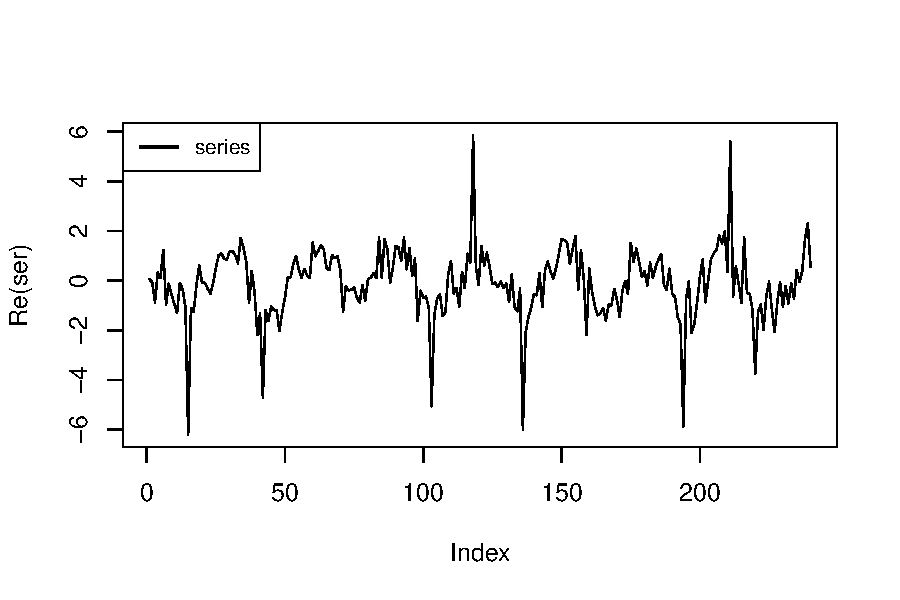
\includegraphics[width=0.67\linewidth]{img/ser_1_Re.png}
	\end{center}
	\caption{Аддитивный ряд. Вещественная часть.}
	\label{ser_Re_1}
\end{figure}

\begin{figure}[H]
	\begin{center}
		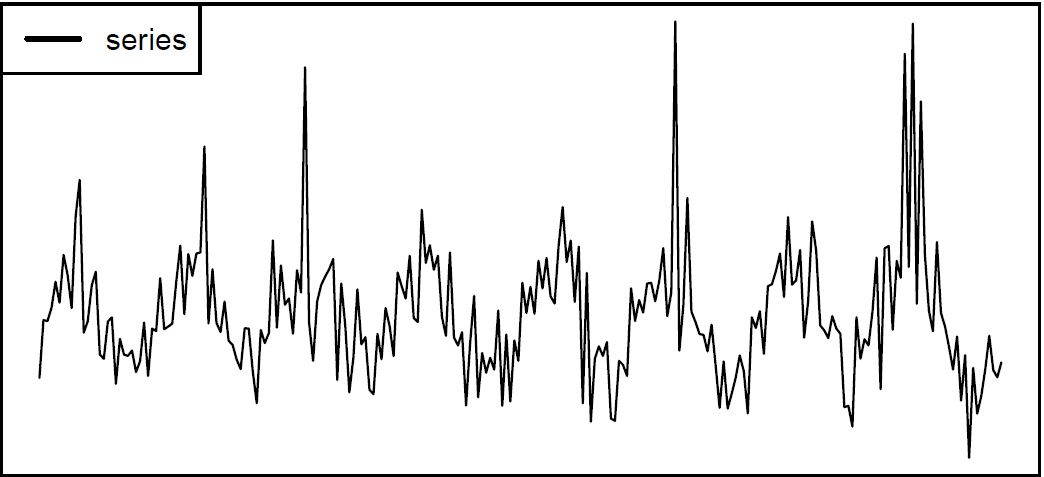
\includegraphics[width=0.67\linewidth]{img/ser_1_Im.png}
	\end{center}
	\caption{Аддитивный ряд. Мнимая часть.}
	\label{ser_Im_1}
\end{figure}

Графики результатов анализа представлены на рис. \ref{analys_Re_1} и \ref{analys_Im_1}. В таблице \ref{tab2} представлены сравнения ошибок для различных методов.  В таблице \ref{tab: pval2} представлены p-value для сравнения методов с лучшим. Длина окна взята $L = 120$.

\begin{figure}[H]
	\begin{center}
		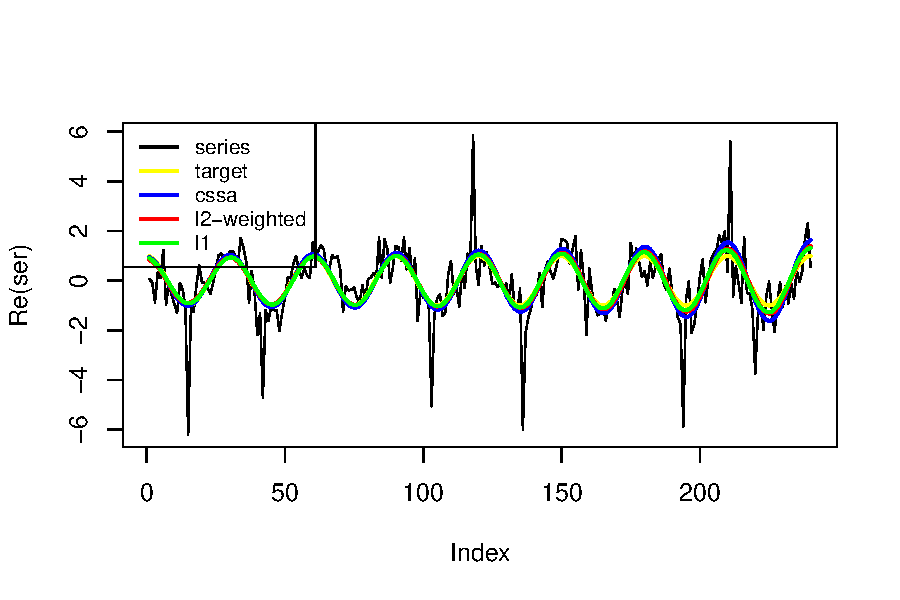
\includegraphics[width=0.67\linewidth]{img/analys_1_Re.png}
	\end{center}
	\caption{Аддитивный ряд. Вещественная часть выделения тренда.}
	\label{analys_Re_1}
\end{figure}

\begin{figure}[H]
	\begin{center}
		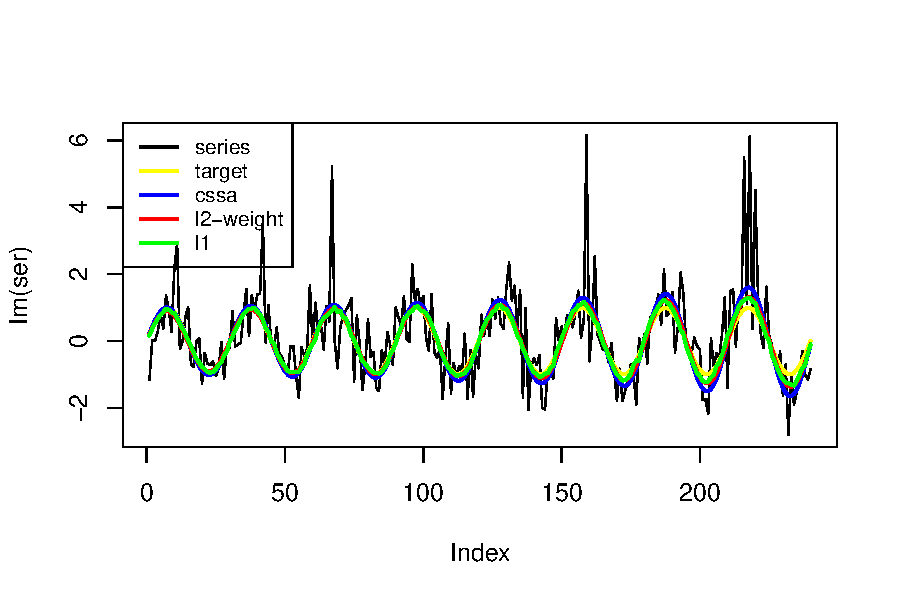
\includegraphics[width=0.67\linewidth]{img/analys_1_Im.png}
	\end{center}
	\caption{Аддитивный ряд. Мнимая часть выделения тренда.}
	\label{analys_Im_1}
\end{figure}

\begin{table}[H]
	\begin{center}
		\caption{Аддитивный ряд с выбросами. Оценки RMSE.}
		\label{tab2}
		\begin{tabular}{|c|c|c|c|c|c|c|}
			\hline
			Method 	& CSSA & L1 & weighted L2 & loess L2 & median L2 & lowess L2 \\
			\hline
			RMSE & 0.285  & 0.147  & 0.158 & $\mathbf{0.112}$ & 0.114 & 0.114\\
			\hline
		\end{tabular}
	\end{center}
\end{table}

\begin{table}[H]
	\caption{Аддитивный ряд с выбросами. p-value сравнения с наилучшим loess L2.}
	\label{tab: pval2}
	\begin{center}
		\begin{tabular}{|c|c|c|c|c|c|}
			\hline
			Method & CSSA	& L1 & weighted L2 & median L2 & lowess L2  \\
			\hline
			p-value & 0  & 7.7e-13 &   4.1e-10  &  \textbf{0.134} & \textbf{0.262}  \\
			\hline
		\end{tabular} \\
	\end{center}
\end{table}

В случае наличия выбросов метод loess L2 показал наилучший результат, за исключением того, что сравнения с другими вариациями модифицированной взвешенной проекции незначимы.


\subsubsection{Мультипликативная модель ряда}

Рассмотрим сигнал с растущей амплитудой и шум с непостоянной дисперсией, пропорциональной сигналу.
Длину ряда возьмём $N = 240$
$$x_n = e^{4n/N} e^{\iu 2n\pi/30} + \frac{1}{2}e^{4n/N} \varepsilon_n, ~ \varepsilon_n \sim CN(0,1).$$
Рассмотрим результаты работы методов для такого ряда (таблица \ref{tab3}).  В таблице \ref{tab: pval3} представлены p-value для сравнения методов с лучшим. Ранг ряда равен 1. RMSE считается по 30 реализациям ряда.

\begin{table}[H]
	\begin{center}
		\caption{Мультипликативный ряд без выбросов. Оценки RMSE.}
		\label{tab3}
		\begin{tabular}{|c|c|c|c|c|c|c|}
			\hline
			Method 	& CSSA & L1 & weighted L2 & loess L2 & median L2 & lowess L2 \\
			\hline
			RMSE & $\mathbf{1.28}$  & 1.52  & 1.90 & 1.36 & 1.43 & 1.37\\
			\hline
		\end{tabular}
	\end{center}
\end{table}

\begin{table}[H]
	\caption{Мультипликативный ряд без выбросов. p-value сравнения методов с наилучшим CSSA.}
	\label{tab: pval3}
	\begin{center}
		\begin{tabular}{|c|c|c|c|c|c|}
			\hline
			Method & L1 & weighted L2 & loess L2 & median L2 & lowess L2  \\
			\hline
			p-value & 0.005   & 0.0001 & 0.001  & 7.6e-5 & 0.0007  \\
			\hline
		\end{tabular} \\
	\end{center}
\end{table}

В случае отсутствия выбросов лучший результат показывает CSSA. Здесь же видно, что модифицированный метод взвешенной проекции справляется с не стационарным рядом куда лучше чем weighted L2, к примеру, сравнивая weighted L2 и loess, сравнение является значимым с p-value $ = 0.0005$.

Теперь добавим к ряду $5\%$ выбросов с величиной выброса $5x_i$. Графики ряда представлены на рис. \ref{ser_Re_2} и \ref{ser_Im_2}.

\begin{figure}[H]
	\begin{center}
		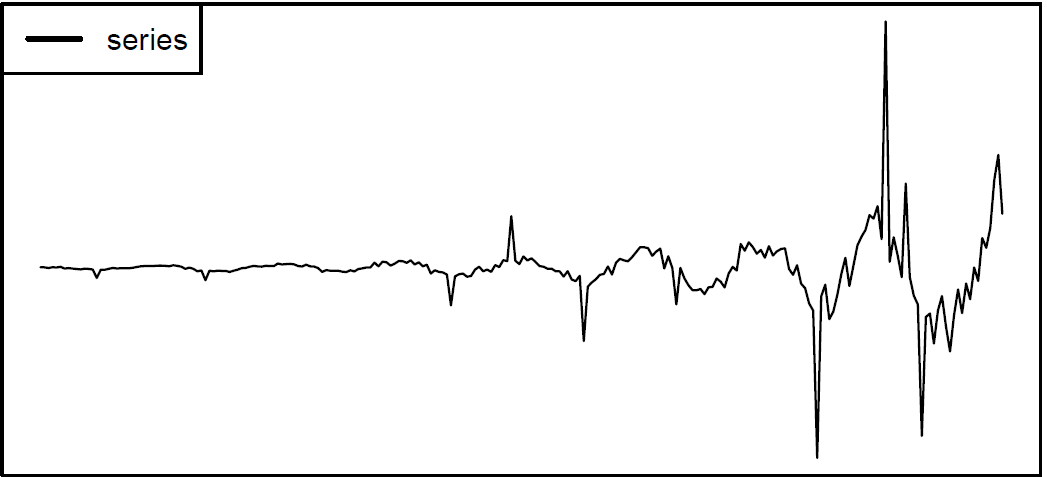
\includegraphics[width=0.67\linewidth]{img/ser_2_Re.png}
		\caption{Мультипликативный ряд. Вещественная часть.}
		\label{ser_Re_2}
	\end{center}
\end{figure}

\begin{figure}[H]
	\begin{center}
		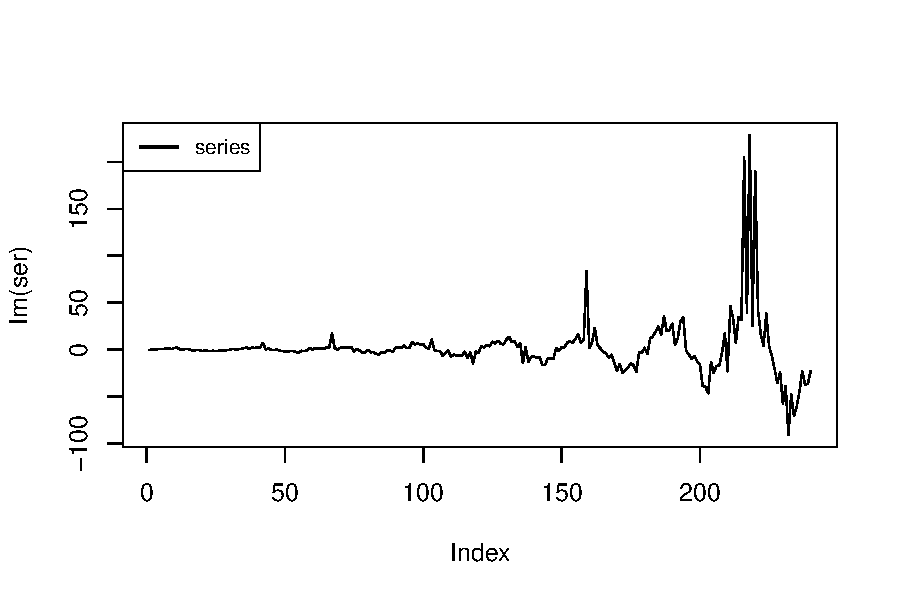
\includegraphics[width=0.67\linewidth]{img/ser_2_Im.png}
		\caption{Мультипликативный ряд. Мнимая часть.}
		\label{ser_Im_2}
	\end{center}
\end{figure}

Графики результатов анализа представлены на рис. \ref{analys_Re_2} и \ref{analys_Im_2}. В таблице \ref{tab4} представлены сравнения ошибок для различных методов. В таблице \ref{tab: pval4} представлены p-value для сравнения методов с лучшим. Длина окна взята $L = 120$.

\begin{figure}[H]
	\begin{center}
		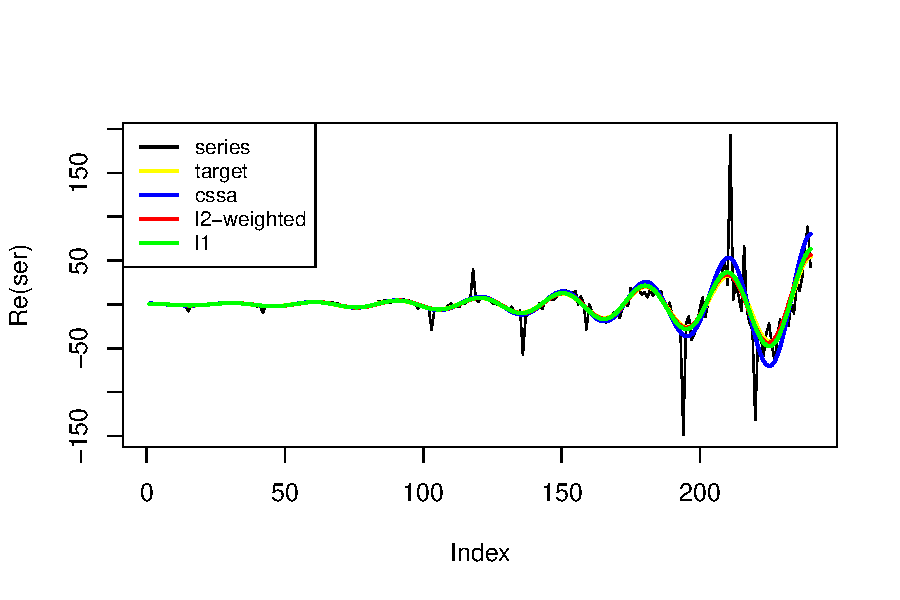
\includegraphics[width=0.67\linewidth]{img/analys_2_Re.png}
		\caption{Мультипликативный ряд. Вещественная часть выделения тренда.}
		\label{analys_Re_2}
	\end{center}
\end{figure}

\begin{figure}[H]
	\begin{center}
		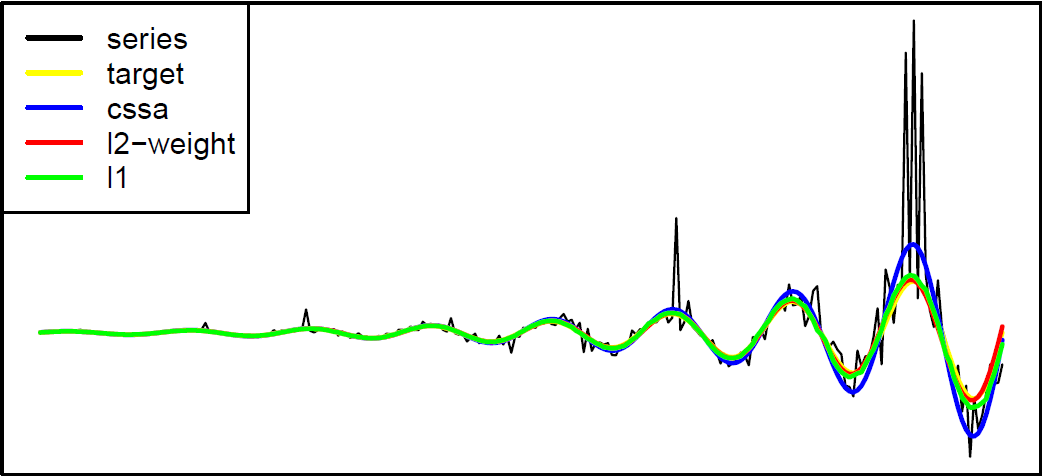
\includegraphics[width=0.67\linewidth]{img/analys_2_Im.png}
		\caption{Мультипликативный ряд. Мнимая часть выделения тренда.}
		\label{analys_Im_2}
	\end{center}
\end{figure}

\begin{table}[H]
	\begin{center}
		\caption{Мультипликативный ряд с выбросами. Оценки RMSE.}
		\label{tab4}
		\begin{tabular}{|c|c|c|c|c|c|c|}
			\hline
			Method 	& CSSA & L1 & weighted L2 & loess L2 & median L2 & lowess L2 \\
			\hline
			RMSE & 6.14  & 1.78  & 1.66 & $\mathbf{1.48}$ & 1.50 & 1.49\\
			\hline
		\end{tabular}
	\end{center}
\end{table}

\begin{table}[H]
	\caption{Мультипликативный ряд с выбросами. p-value сравнения методов с наилучшим loess L2.}
	\label{tab: pval4}
	\begin{center}
		\begin{tabular}{|c|c|c|c|c|c|}
			\hline
			Method & CSSA	& L1 & weighted L2 & median L2 & lowess L2  \\
			\hline
			p-value & 3.5e-16   & 0.005 &   \textbf{0.13}  &  \textbf{0.387} & \textbf{0.28}  \\
			\hline
		\end{tabular} \\
	\end{center}
\end{table}

В случае присутствия выбросов loess L2 показывает себя наилучшим образом на данном примере, однако сравнения с weighted L2, median~\ L2 и lowess L2 не являются значимыми.

Приведённые примеры подтверждают эффективность робастных модификаций CSSA, с точки зрения RMSE. Помимо этого, была подтверждена эффективность модификации weighted L2 (конкретной, loess L2) для рядов с гетероскедастичным шумом. Однако, требуется исследовать трудоёмкость методов, для более полного ответа на вопрос, какой из них более предпочтителен в конкретной ситуации.

\subsection{Сравнение вещественного и комплексного подхода} \label{sec:comp}

В данной работе вещественные алгоритмы, представленные в \cite{Tretyakova20}, были обобщены на комплексный случай. Зная, что комплексное число раскладывается на две вещественные компоненты, вещественную и мнимую части, возможно использовать вещественные алгоритмы для выделения сигнала отдельно из вещественной и мнимой частей ряда. Второй же подход~--- использовать комплексный алгоритм для всего ряда.

Сравним оба этих подхода на примере.
Длину ряда возьмём $N = 50$, $L = 20$
$$x_n = \cos(2n\pi/10) + \iu\cos(2n\pi/10 + \phi) + \varepsilon_n, ~ \varepsilon_n \sim CN(0,0.01).$$
добавим к ряду выброс с величиной выброса $5x_i$ на позиции $N/2$,

Будем сравнивать MSE для комплексных и вещественных алгоритмов на 100 повторах.
Обозначим метод CSSA(SSA) как базовый метод для робастных модификаций за Basic.
Результаты сравнения MSE для $\phi = \pi / 4$ приведены в таблице \ref{tab:th_ex}.
\begin{table}[H]
	\caption{MSE, $\phi = \pi / 4$.}
	\label{tab:th_ex}
	\begin{center}
		\begin{tabular}{|c|c|c|c|c|}
			\hline
			Метод & Ряд & Basic & weighted L2 & median L2\\
			\hline
			CSSA & $\tX$ & 0.064 & 0.0011 & 0.0012\\
			\hline
			SSA & $\Re(\tX)$ & 0.042 & 0.0006 &   0.0006\\
			\hline
			SSA & $\Im(\tX)$ & 0.022   & 0.0006 &   0.0006\\
			\hline
		\end{tabular} \\
	\end{center}
\end{table}

Из таблицы видно, что, с точки зрения MSE для данного сигнала оба подхода эквивалентны (MSE для комплексного алгоритма равно суммарному MSE для двух применений вещественного алгоритма). Откуда возникает подобный эффект и для каких сигналов он наблюдается, рассмотрим в следующей главе.

Приведём аналогичный пример, но с комплексной экспонентой. Результаты в таблице \ref{tab:th_ex_exp}.

\begin{table}[H]
	\caption{MSE, $\phi = \pi / 2$.}
	\label{tab:th_ex_exp}
	\begin{center}
		\begin{tabular}{|c|c|c|c|c|}
			\hline
			Метод & Ряд & Basic & weighted L2 & median L2 \\
			\hline
			CSSA & $\tX$ & 0.021 & 0.0006 & 0.0006\\
			\hline
			SSA & $\Re(\tX)$ & 0.042 & 0.0006 &   0.0006\\
			\hline
			SSA & $\Im(\tX)$ & 0.0006   & 0.0006 &   0.0006\\
			\hline
		\end{tabular} \\
	\end{center}
\end{table}

Из таблицы~\ref{tab:th_ex_exp} видно, что CSSA даёт вдвое меньшую ошибку, чем суммарная ошибка для SSA.

\subsubsection{Вещественные выбросы}
Посмотрим, изменится ли что-то, если рассмотреть те же ряды, но с вещественными выбросом величины $5|x_i|$ на позиции $N/2$.

Результаты сравнения MSE приведены в таблицах \ref{tab:re_outl} и \ref{tab:re_outl_exp}.
\begin{table}[H]
	\caption{MSE, $\phi = \pi/4$.}
	\label{tab:re_outl}
	\begin{center}
		\begin{tabular}{|c|c|c|c|c|}
			\hline
			Метод & Ряд & Basic & weighted L2 & median L2\\
			\hline
			CSSA & $\tX$ & 0.066 & 0.0011 & 0.0012\\
			\hline
			SSA & $\Re(\tX)$ & 0.066 & 0.0005 &   0.0006\\
			\hline
			SSA & $\Im(\tX)$ & 0.0006   & 0.0006 &   0.0006\\
			\hline
		\end{tabular} \\
	\end{center}
\end{table}

\begin{table}[H]
	\caption{MSE, $\phi = \pi/2$.}
	\label{tab:re_outl_exp}
	\begin{center}
		\begin{tabular}{|c|c|c|c|c|}
			\hline
			Метод & Ряд & Basic & weighted L2 & median L2\\
			\hline
			CSSA & $\tX$ & 0.022 & 0.006 & 0.0006\\
			\hline
			SSA & $\Re(\tX)$ & 0.044 & 0.0006 &   0.0007\\
			\hline
			SSA & $\Im(\tX)$ & 0.0006   & 0.0006 &   0.0006\\
			\hline
		\end{tabular} \\
	\end{center}
\end{table}

Заметим, что предыдущие наблюдения сохраняются и, более того, сохраняется ошибка для CSSA.

\chapter{Ошибка оценки сигнала в SSA и CSSA}
\label{ch:perturb}
В предыдущей главе рассматривались модификации метода CSSA для рядов с выбросами.
Однако, комплексный временной ряд представляется через свою вещественную и мнимую части, к каждой из которых можно применить вещественный метод и, таким образом, получить оценку комплексного сигнала. Исходя из этого возникает вопрос, насколько полезны комплексные обобщения методов? В данном разделе мы постараемся ответить на данный вопрос с точки зрения ошибок восстановления на примере сравнения базовых вариантов методов CSSA и SSA.

Пусть наблюдаемый комплексный временной ряд имеет вид $\tX =\tS + \tR$. Для получения оценки сигнала будем использовать метод CSSA. Кроме применения CSSA ко всему ряду будем также применять метод SSA отдельно к вещественной и мнимой части ряда $\tX$.

Для анализа ошибки оценивания сигнала используется теория возмущений \cite{Kato}, которая была применена для случая выделения сигнала методом SSA в ряде работ, см., например, \cite{Nekrutkin}.
Хотя теория возмущения Като дает вид полной ошибки, однако ее исследование представляется сложной задачей. Поэтому мы будем рассматривать только первый порядок ошибки в разложении ошибки по величине возмущения.
При этом проведем численное сравнение первого порядка ошибки и полной ошибки для выявления случаев, когда анализ первого порядка ошибки плохо описывает полную ошибку и поэтому его анализ не представляет интереса.

Даже для первого порядка ошибки получение его явного вида --- довольно трудоемкая задача. Нам удалось его получить для случая константного сигнала и возмущения в виде выброса. В общем случае результаты касаются сравнения MSE ошибок оценки сигнала методом CSSA и суммарного MSE при применении SSA отдельно к мнимой и вещественной частям.


\section{Применение теории возмущений к SSA и CSSA}
% и \cite{Konstantinov}

Рассматриваем временной ряд $\tX=(x_1, \ldots, x_{N})$, $L$ --- длина окна, $r$ --- ранг оцениваемого сигнала (ранг траекторной матрицы сигнала).

Напомним, как будет выглядеть оценка сигнала для SSA(CSSA)
	\begin{equation*}
		\tilde{\tS} = \mathcal{T}^{-1}_{L} \Pi_{\mathcal{H}} \Pi_{r} \mathcal{T}_L (\tX).
	\end{equation*}

Рассмотрим $\tX = \tS(\delta)$, где $\tS(\delta) = \tS + \delta \tR$ длины $N$, $\mathbf{H} = \mathcal{T}_L(\tS)$.

Из \cite{Nekr2008} известно следующее представление $\tilde{\tS} = \mathcal{T}_L^{-1} \Pi_{\mathcal{H}} (\mathbf{H} + \delta\mathbf{H}^{(1)} + \delta^2\mathbf{H}^{(2)})$.

Ошибку восстановления обозначим как $\tF = \tilde{\tS} - \tS = \mathcal{T}_L^{-1} \Pi_{\mathcal{H}} (\delta\mathbf{H}^{(1)} + \delta^2\mathbf{H}^{(2)})$.

Рассмотрим $\delta = 1$ и $\tX = \tS + \tR$. Первый порядок ошибки восстановления обозначим как $\tF^{(1)} = \mathcal{T}_L^{-1} \Pi_{\mathcal{H}}(\mathbf{H}^{(1)})$.

\begin{statement} \label{st:main}
	
	Обозначим $\mathbf{E}(\delta) = \mathcal{T}_L(\delta \tR)$ и рассмотрим $\delta_0 > 0$. Если
	\begin{equation} \label{eq:main_cond}
		\|\mathbf{E}(\delta)\| < \mu_{\min} / 2
	\end{equation}
	для любого $\delta \in (-\delta_0, \delta_0)$, где $\mu_{\min}$~--- минимальное сингулярное число $\mathbf{H}$, то
\begin{equation} \label{eq:main}
	\mathbf{H}^{(1)} = \mathbf{P}^{\perp}_0 \mathbf{E} \mathbf{Q}_0 + \mathbf{P}_0 \mathbf{E},
\end{equation}
где $\mathbf{P}_0$~--- проектор на пространство столбцов $\mathbf{H}$, $\mathbf{Q}_0$~--- проектор на пространство строк $\mathbf{H}$, $\mathbf{P}^{\perp}_0 = \mathbf{I} - \mathbf{P}_0$, $\mathbf{I}$~--- единичная матрица, $\mathbf{E} = \mathcal{T}_L(\tR)$.
\end{statement}
\begin{proof}
	
По теореме 2.1 из \cite{Nekrutkin}, при выполнении \eqref{eq:main_cond} верно
\begin{equation} \label{eq:main_proof_1}
\delta\mathbf{H}^{(1)} = \mathbf{W}_1(\delta) \mathbf{H}(\delta) + \delta \mathbf{P}_0 \mathbf{E},
\end{equation}
где $\mathbf{H}(\delta) = \mathcal{T}_L(\tS(\delta))$.
Из \cite[стр.12]{Konstantinov} известно
\begin{equation} \label{eq:main_proof_2}
	\mathbf{W}_1(\delta) \mathbf{H}(\delta) = \delta \mathbf{P}^{\perp}_0 \mathbf{E} \mathbf{Q}_0.
\end{equation}
Используя \eqref{eq:main_proof_1}, \eqref{eq:main_proof_2} и сокращая на $\delta$, получаем
\begin{equation*}
	\mathbf{H}^{(1)} = \mathbf{P}^{\perp}_0 \mathbf{E} \mathbf{Q}_0 + \mathbf{P}_0 \mathbf{E}.
\end{equation*}
\end{proof}

В дальнейшем будем писать достаточно малое возмущение $\tR$, понимая под этим выполнение \eqref{eq:main_cond}.

\subsection{Сравнение CSSA и SSA в случае совпадающих пространств сигналов}

Обозначим за:

$\tF^{(1)} = \mathcal{H}(\mathbf{H}^{(1)}(\tR, \tS))$ первый порядок ошибки восстановления $\tS$ с возмущением $\tR$ метода CSSA,

$\tF^{(1)}_{\Re} = \mathcal{H}(\mathbf{H}^{(1)}(\Re(\tR), \Re(\tS)))$ первый порядок ошибки восстановления $\Re(\tS)$ с возмущением $\Re(\tR)$ метода SSA,

$\tF^{(1)}_{\Im} = \mathcal{H}(\mathbf{H}^{(1)}(\Im(\tR), \Im(\tS)))$ первый порядок ошибки восстановления $\Im(\tS)$ с возмущением $\Im(\tR)$ метода SSA.


\begin{theorem}\label{th:sum}
	Пусть пространства столбцов траекторных матриц рядов $\tS$, $\Re(\tS)$ и $\Im(\tS)$ совпадают и то же самое верно для пространств строк.
	Тогда при любом достаточно малым возмущении $\tR$ $$\tF^{(1)} = \tF^{(1)}_{\Re} + \iu\tF^{(1)}_{\Im}.$$
\end{theorem}
\begin{proof}
	Рассмотрим матрицу возмущения $\mathbf{E} = \Re(\mathbf{E}) + \iu\Im(\mathbf{E}).$
	Заметим, что в \eqref{eq:main} $\mathbf{E}$ входит линейно, поэтому
	\begin{equation} \label{eq_reim}
		\mathbf{H}^{(1)}(\tR, \tS) = \mathbf{H}^{(1)}(\Re(\tR), \tS) + \iu\mathbf{H}^{(1)}(\Im(\tR), \tS).
	\end{equation}
	Тогда из \eqref{eq_reim}, линейности диагонального усреднения и  совпадения траекторных пространств получаем
	\begin{multline*}
		\tF^{(1)} = \mathcal{H}(\mathbf{H}^{(1)}(\tR, \tS)) = \mathcal{H}(\mathbf{H}^{(1)}(\Re(\tR), \tS)) + \iu\mathcal{H}(\mathbf{H}^{(1)}(\Im(\tR), \tS)) =\\
		\mathcal{H}(\mathbf{H}^{(1)}(\Re(\tR), \Re(\tS))) + \iu\mathcal{H}(\mathbf{H}^{(1)}(\Im(\tR), \Im(\tS))) = \tF^{(1)}_{\Re} + \iu\tF^{(1)}_{\Im}	
	\end{multline*}
	
\end{proof}

Заметим, что хотя в утверждении теоремы возмущение $\tR$ может быть любым по форме, однако теорема имеет практическое применение, только если первый порядок ошибки адекватно описывает полную ошибку.

%\begin{notice*}
%	Требования теоремы означают существование вещественного базиса в пространстве столбцов $\mathbf{H}$$\mathbf{H}^{\mathrm{H}}$.
%\end{notice*}

%\begin{notice*}
%	Примером сигнала, для которого в общем случае очевидно не выполняются требования теоремы, %является комплексная экспонента $s_n = e^{\phi(n) + i\psi(n)}$, поскольку $\rk S = 1$, а %$\rk\Re(S) = \rk\Im(S) = 2$.
%\end{notice*}


\subsubsection{Случайное возмущение}

Рассмотрим случайное возмущение $\tR$.

Для дальнейших рассуждений приведём известный результат.
\begin{lemma} \label{std:disp}
	Пусть $\zeta = \xi + \iu\eta$. Тогда $\mathbb{D}\zeta = \mathbb{D}\xi + \mathbb{D}\eta$.
\end{lemma}
\begin{proof}
\begin{multline*}
	\mathbb{D}\zeta = \mathbb{E}(|\zeta - \mathbb{E}\zeta|^2) = \mathbb{E}(|(\xi - \mathbb{E}\xi) + \iu((\eta - \mathbb{E}\eta))|^2) = \\
	= \mathbb{E}((\xi - \mathbb{E}\xi)^2 + (\eta - \mathbb{E}\eta)^2)= \mathbb{E}(\xi - \mathbb{E}\xi)^2 + \mathbb{E}(\eta - \mathbb{E}\eta)^2 = \mathbb{D}\xi + \mathbb{D}\eta.
\end{multline*}
\end{proof}

Рассмотрим первые порядки ошибок восстановления сигнала:

$\tF^{(1)} = (f^{(1)}_1, \ldots, f^{(1)}_N)$, $\tF^{(1)}_{\Re} = (f^{(1)}_{\Re,1}, \ldots, f^{(1)}_{\Re, N})$, $\tF^{(1)}_{\Im} = (f^{(1)}_{\Im,1}, \ldots, f^{(1)}_{\Im, N})$.


\begin{corollary}[из теоремы {\ref{th:sum}}] \label{st:dispsum}
	Пусть выполнены условия теоремы \ref{th:sum}.
	Тогда для любого $l$, $1\le l \le N$,
	\begin{equation} \label{eq:dispsum}
		\mathbb{D}f^{(1)}_l = \mathbb{D}f^{(1)}_{\Re, l} + \mathbb{D}f^{(1)}_{\Im, l}.	
	\end{equation}
\end{corollary}

Утверждение получается автоматически из теоремы \ref{th:sum} и леммы \ref{std:disp}.

\subsubsection{Возмущение в виде выброса} \label{ss:RMSEinv}

Рассмотрим возмущение выбросом $a_1 + \iu a_2$ на позиции $k$, т.е. ряд $\tR$ состоит из нулей кроме значения $a_1 + \iu a_2$ на $k$-м месте.
Возмущение выбросом $a_1 + \iu a_2$ можно записать как  $\tR = (a_1 + \iu a_2)\tG$, где $\tG$~--- ряд, равный $1$ на $k$-м месте, а все остальные его элементы нулевые.

\begin{statement}\label{st:RMSEinv}
	Пусть возмущение выбросом $a_1 + \iu a_2$ на позиции $k$ достаточно мало.
	Тогда $|f_l^{(1)}|$ для ряда с сигналом $\tS$ и выбросом $a_1 + \iu a_2$ на позиции $k$, и  ряда с сигналом $\tS$ и выбросом $b_1 + \iu b_2$ на позиции $k$, таким что $|b_1 + \iu b_2| = |a_1 + \iu a_2|$, совпадают для любого $l$, $1\le l \le N$.
\end{statement}
\begin{proof}
	Используем представление $\tR = (a_1 + \iu a_2)\tG$.
	По формуле \eqref{eq:main}
	$$f^{(1)}_l = (a_1 + \iu a_2)\mathcal{H}(\tG, \tS)_l = (a_1 + \iu a_2)c_l.$$
	Для ряда с сигналом $S$ и выбросом $a_1 + \iu a_2$ на позиции $k$ имеем
	$$|f^{(1)}_l| = |(a_1 + \iu a_2)c_l| = |a_1 + \iu a_2|\cdot|c_l|. $$
	Рассмотрим выброс $b_1 + \iu b_2$, такой что $|b_1 + \iu b_2| = |a_1 + \iu a_2|$.
	Для ряда с сигналом $\tS$ и выбросом $b_1 + \iu b_2$ на позиции $k$ получаем
	$$|f^{(1)}_l| = |(b_1 + \iu b_2)c_l| = |b_1 + \iu b_2|\cdot|c_l| = |a_1 + \iu a_2|\cdot|c_l|. $$
\end{proof}

Данное утверждение объясняет, почему в численных экспериментах раздела \ref{sec:comp} сохраняется ошибка CSSA при изменении выброса.

%\subsection{Частный случай}
%Рассматриваем ряд с $s_n = c_1 + ic_2$ и матрицу шума $\mathbf{E}$ с дисперсиями вещественной и мнимой частей $\sigma_1$ и $\sigma_2$.\\
%Сингулярные векторы такого ряда являются нормированными векторами с одинаковыми компонентами, они также сингулярные для вещественной и мнимой части. Тогда выполняются условия теоремы \ref{th:sum} и
%
%$$f^{(1)} = f^{(1)*}_{\Re(S)} + if^{(1)*}_{\Im(S)}.$$
%
%В данном случае $\Re(S)$ и $\Im(S)$ являются вещественными константами.
%
%В работе \cite{Vlas2008} была получена аналитическая формула для дисперсии каждого элемента вещественных констант, в нашем случае $f^{(1)*}_{\Re}$ и $f^{(1)*}_{\Im}$.
%
%Обозначим $L = \alpha N$, $\alpha \leq \frac{1}{2}$, $\lambda = \lim_{N\to\infty} 2 l / N$, воспользовавшись утверждением \ref{st:dispsum}, получаем
%
%$$
%\mathbb{D} f^{(1)}_l = \mathbb{D} f^{(1)*}_{\Re, l} + \mathbb{D} f^{(1)*}_{\Im, l} \sim \frac{\sigma^2_1 + \sigma^2_2}{N}
%\begin{cases}
%	D_1(\alpha, \lambda), &\text{$0 \leq \lambda \leq 2 (1 - 2\alpha)$}\\
%	D_2(\alpha, \lambda), &\text{$2 (1 - 2\alpha) < \lambda < 2\alpha$}\\
%	D_3(\alpha, \lambda), &\text{$2\alpha \leq \lambda \leq 1$}
%\end{cases},
%$$
%где
%\begin{gather*}
%	D_1(\alpha, \lambda) = \frac{1}{12 \alpha^2(1 - \alpha)^2} (\lambda^2(\alpha + 1) - 2\lambda\alpha(1 + \alpha)^2 + 4 \alpha(-3\alpha + 3 + 2\alpha^2))\\
%	D_3(\alpha, \lambda) = \frac{1}{6 \alpha^2\lambda^2 (\alpha - 1)} (\lambda^4 + 2\lambda^3(3\alpha -2 -3\alpha^2) + \\
%	+ 2\lambda^2(3 - 9\alpha + 12\alpha^2 - 4\alpha^3) + 4\lambda(4 \alpha^4 - 4\alpha^3 - 3\alpha^2 + 4\alpha - 1) +\\
%	+ 8\alpha - 56 \alpha^2 + 144\alpha^3 - 160\alpha^4 + 64\alpha^5\\
%	D_3(\alpha, \lambda) = \frac{2}{3\alpha}.\\
%\end{gather*}
%
%Формулы выписаны только до середины ряда из симметричности дисперсии первого порядка ошибки относительно середины ряда.

\subsection{Случай двух зашумленных синусоид}
Пусть сигнал $\tS = (s_1, \ldots, s_N)$ имеет вид
\begin{equation}
	\label{eq:general_ts}
	s_l = A\cos(2 \pi\omega l + \phi_1) + \iu B\cos(2 \pi\omega l + \phi_2),
\end{equation}
где $0<\omega < 0.5$ и $0\le\phi_i < 2\pi$.
Заметим, что случай $|\phi_1-\phi_2| = \pi/2\,(\mmod \pi)$ и $A=B$ соответствует комплексной экспоненте.

Пусть возмущение $\tR$~--- шум, т.е. случайный вектор с нулевым математическим ожиданием и достаточно малой дисперсией.

\begin{corollary}[из теоремы {\ref{th:sum}}] \label{cor:harm}
	Для комплексного ряда вида \eqref{eq:general_ts}, кроме случая $|\phi_1-\phi_2| = \pi/2\,(\mmod \pi)$ и $A=B$,  выполняется равенство \eqref{eq:dispsum}.
\end{corollary}
Выполнение условий теоремы {\ref{th:sum}} (совпадение столбцовых и строковых траекторных пространств сигналов) уже было показано (см. утверждение \ref{st:L-rk}).

\begin{remark}
	Численные эксперименты, проведённые в \cite{Golyandina.etal2013}, показывают, что для сигнала в виде вида \eqref{eq:general_ts}, не являющегося комплексной экспонентой, суммарная MSE CSSA-оценки сигнала равна сумме суммарных MSE SSA-оценок сигнала его вещественной и мнимой частей. Следствие \ref{cor:harm} является теоретическим объяснением данного результата.
\end{remark}

Наиболее распространённым видом сигналов в случае комплексных временных рядов, встречающихся на практике, является комплексная экспонента. Однако, по утверждению \ref{st:L-rk} условия теоремы \ref{th:sum} для такого сигнала не выполняются. А, соответственно, и формула \eqref{eq:dispsum} не применима.

\begin{prop*}
	Для случая комплексной экспоненты, с возмущением $\tR$ выполняется
	\begin{equation} \label{eq:expdisp}
		\mathbb{D}(f^{(1)}_l) \stackrel{?}{=} \frac{1}{2}[\mathbb{D}(f^{(1)}_{\Re, l}) + \mathbb{D}(f^{(1)}_{\Im, l})].
	\end{equation}
\end{prop*}

Формула \eqref{eq:expdisp} была проверена числено. Приведём пример подобной проверки, рассмотрим сигнал
$$s_l = e^{\iu 2 \pi l / 10},$$
параметры $\sigma^2 = 0.01$, $N = 5$, $L = 3$.

Результаты представлены в таблице~\ref{tab:pi_div_2}.

\begin{table}[H]
	\begin{center}
		\caption{Оценки дисперсий при $10^3$ повторах.}
		\label{tab:pi_div_2}
		\begin{tabular}{|c|c|c|c|c|c|}
			\hline
			$l$	& 1 & 2 & 3 & 4 & 5\\
			\hline
			$\hat{\mathbb{D}}(f^{(1)}_l)$ & 0.013  & 0.008  & 0.005 & 0.008 & 0.014\\
			\hline
			$\hat{\mathbb{D}}(f^{(1)}_{\Re, l})$ & 0.010 & 0.008 & 0.006 & 0.008 & 0.010\\
			\hline
			$\hat{\mathbb{D}}(f^{(1)}_{\Im, l})$ & 0.010  & 0.007  & 0.006 & 0.008 & 0.010\\
			\hline
		\end{tabular}
	\end{center}
\end{table}

Из таблицы можно заметить приближённое численное выполнение \eqref{eq:expdisp}, за исключением крайних точек. Это объясняется малой длиной ряда, ввиду медленной сходимости по длине ряда на краях.

\subsection{Случай константных сигналов с выбросом}
Рассматриваем сигнал $\tS = (c_1 + \iu c_2, \ldots, c_1 + \iu c_2)$, возмущённый выбросом $a_1 + \iu a_2$ на позиции $k$, т.е. ряд $\tR$ состоит из нулей кроме значения $a_1 + \iu a_2$ на $k$-м месте. Исходя из теоремы \ref{th:sum}, достаточно уметь вычислять первый порядок ошибки восстановления сигнала $\tS = (c, \ldots, c)$, возмущённого выбросом $a$ на позиции $k$.

В работе \cite{Nekr2008} была получен частный случай формулы \eqref{eq:main} для вещественных сигналов единичного ранга:
\begin{equation} \label{eq:real_rk1}
\mathbf{H}^{(1)}(\tR, \tS) = -U^{\mathrm{T}} \mathbf{E} V U V^{\mathrm{T}} + U U^{\mathrm{T}} \mathbf{E} + \mathbf{E} V V^{\mathrm{T}} = -\mathbf{I}_1 + \mathbf{I}_2 + \mathbf{I}_3,
\end{equation}
где $U$, $V$~--- сингулярные векторы матрицы $\mathbf{H}$.

Матрица возмущения для выброса $a$ имеет вид
$$\mathbf{E}^{\mathrm{T}} = \begin{pmatrix}
	0 & 0 & 0 & \ldots &  a  & \ldots & 0\\
	 \vdots &\vdots & \vdots & &  \vdots & & \vdots\\
	0 & 0 & a & \ldots & 0 & \ldots & 0\\
	0 & a & 0 & \ldots & 0 & \ldots & 0\\
	a & 0 & 0 & \ldots & 0 & \ldots & 0\\
	\vdots &\vdots & \vdots & & \vdots & & \vdots\\
	0 & 0 & 0 & \ldots & 0 & \ldots & 0\\
\end{pmatrix} \in \mathbb{R}^{K \times L}.$$

Для сигнала $\tS = (c, \ldots, c)$ сингулярные вектора имеют вид
$U = \{1/\sqrt{L}\}^{L}_{i = 1},\, V = \{1/\sqrt{K}\}^{K}_{i = 1}$, $K = N - L + 1$,
Не умаляя общности, будем считать, что $L \leq K$.

\subsubsection{Случай $1 \leq k < L$}

Рассмотрим члены суммы из формулы \eqref{eq:real_rk1} покомпонентно.

Найдём $\mathbf{I}_1$:
$$U^{\mathrm{T}} \mathbf{E} = \begin{pmatrix}
	 a/\sqrt{L} & \ldots & a/\sqrt{L} & 0 & \ldots & 0\\
\end{pmatrix},$$

$$U^{\mathrm{T}} \mathbf{E} V = k a / \sqrt{LK},$$

$$U V^{\mathrm{T}} = \begin{pmatrix}
	1/\sqrt{LK} & \ldots & 1/\sqrt{LK}\\
	\vdots & & \vdots\\
	1/\sqrt{LK} &   \ldots &  1/\sqrt{LK}
\end{pmatrix}\in \mathbb{R}^{L \times K}
,$$

$$\mathbf{I}_1 = U^{\mathrm{T}} \mathbf{E} V U V^{\mathrm{T}} = \begin{pmatrix}
	k a/ LK & \ldots &  k a/ LK\\
	\vdots & & \vdots\\
	k a/ LK &   \ldots &  k a/ LK
\end{pmatrix}.$$

Найдём $\mathbf{I}_2$:
$$U U^{\mathrm{T}} = \begin{pmatrix}
	1/L & \ldots & 1/L\\
	
	\vdots & & \vdots\\
	1/L &   \ldots &  1/L
\end{pmatrix}\in \mathbb{R}^{L \times L},$$

$$\mathbf{I}_2 = U U^{\mathrm{T}} \mathbf{E} = \begin{pmatrix}
	a/L & \ldots & a/L & \ldots & 0\\
	\vdots & & \vdots & & \vdots\\
	a/L & \ldots & a/L & \ldots & 0
\end{pmatrix}.$$

Найдём $\mathbf{I}_3$:
$$V V^{\mathrm{T}} = \begin{pmatrix}
	1/K & \ldots & 1/K\\
	\vdots & & \vdots\\
	1/K &   \ldots &  1/K
\end{pmatrix}\in \mathbb{R}^{K \times K},$$

$$\mathbf{I}_3 = \mathbf{E} V V^{\mathrm{T}} = \begin{pmatrix}
	a/K &  \ldots & a/K\\
	\vdots & & \vdots\\
	a/K &  \ldots & a/K\\
	\vdots & & \vdots\\
	0 & \ldots & 0
\end{pmatrix}.$$

Используя
$$\mathbf{H}^{(1)}(\tR, \tS) = -\mathbf{I}_1 + \mathbf{I}_2 + \mathbf{I}_3,$$
получаем
$$\mathbf{H}^{(1)}(\tR, \tS) = \frac{a}{LK}\begin{pmatrix}
	(L + K - k) & \ldots & (L + K - k) & \ldots & (L - k)\\
	\vdots & & \vdots & & \vdots \\
	(L + K - k) & \ldots & (L + K - k) & \ldots & (L - k) & \\
	\vdots & & \vdots & & \vdots \\
	(K - k) & \ldots & (K - k) & \ldots & -k \\
\end{pmatrix}.$$

Теперь приведём выражение первого порядка ошибки через $\mathbf{H}^{(1)}(\tR, \tS)$
$$\tF^{(1)} = \mathcal{T}_L^{-1} \Pi_{\mathcal{H}}(\mathbf{H}^{(1)}(\tR, \tS)).$$
Получаем формулы для поэлементного выражения первого порядка ошибки восстановления:
\begin{itemize}
\item
$k \leq L/2$

$k \leq K - L$

$$f^{(1)}_l = \frac{a}{{LK}}
\begin{cases}
	(L + K - k), & \text{$1 \leq l \leq k$}\\
	\frac{1}{l}(L + K - l)k, & \text{$k < l \leq L$}\\
	\frac{1}{L}K(L + k - l), &\text{$L < l < L + k$}\\
	0, &\text{$L + k \leq l \leq K$}\\
	\frac{1}{N - l + 1}(K - l)(L - k), &\text{$K < l < K + k$}\\
	-k, &\text{$K + k \leq l \leq N $}
\end{cases}.
$$

\item
$k \leq L/2$

$k > K - L$

$$f^{(1)}_l = \frac{a}{{LK}}
\begin{cases}
	(L + K - k), & \text{$1 \leq l \leq k$}\\
	\frac{1}{l}(L + K - l)k, & \text{$k < l \leq L$}\\
	\frac{1}{L}K(L + k- l), &\text{$L < l < K$}\\
	\frac{1}{N - l + 1}(2KL - l(L + K - k)), &\text{$K \leq l \leq L + k$}\\
	\frac{1}{N - l + 1}( K - l)(L - k), &\text{$L + k < l < K + k$}\\
	-k, &\text{$K + k \leq l \leq N$}
\end{cases}.
$$

\item
$k > L/2$

$k \leq K - L$

$$f^{(1)}_l = \frac{a}{{LK}}
\begin{cases}
	(L + K - k), & \text{$1 \leq l \leq k$}\\
	\frac{1}{l}(L + K - l)k, & \text{$k < l < L$}\\
	%\frac{1}{L}((K + l - 2k)(L - k) + (2k - l)(L + K - k)), & \text{$L\leq l \leq 2k$}\\
	\frac{1}{L}K(L + k - l), &\text{$L \leq l < L + k$}\\
	0, &\text{$L + k \leq l \leq K$}\\
	\frac{1}{N - l + 1}(L - K)(L - k), &\text{$K < l < K + k$}\\
	-k, &\text{$K + k \leq l \leq N$}
\end{cases}.
$$

\item
$k > \max(L / 2, K - L)$

$k \leq K/2$

$$f^{(1)}_l = \frac{a}{{LK}}
\begin{cases}
	(L + K - k), & \text{$1 \leq l \leq k$}\\
	\frac{1}{l}(L + K - l)k, & \text{$k < l < L$}\\
	\frac{1}{L}K(L + k - l), &\text{$L \leq l < K$}\\
	\frac{1}{N - l + 1}(2KL - l(L + K - k)), &\text{$K \leq l \leq L + k$}\\
	\frac{1}{N - l + 1}(L - K)(L - k), &\text{$L + k < l < K + k$}\\
	-k, &\text{$K + k \leq l \leq N$}
\end{cases}.
$$

\item
$k > K/2$


$$f^{(1)}_l = \frac{1}{{LK}}
\begin{cases}
	(L + K - k), & \text{$1 \leq l \leq k$}\\
	\frac{1}{l}(L + K - l)k, & \text{$k < l < L$}\\
	\frac{1}{L}K(L + k - l), &\text{$L \leq l < K$}\\
	\frac{1}{N - l + 1}(2KL - l(L + K - k)), &\text{$K \leq l \leq L + k$}\\
	\frac{1}{N - l + 1}(K - l)(L - k), &\text{$L + k < l < K + k$}\\
	-k, &\text{$K + k \leq l \leq N $}
\end{cases}.
$$
\end{itemize}

\subsubsection{Случай $L \leq k \leq K$}
Аналогично рассмотрим члены суммы из формулы \eqref{eq:real_rk1} покомпонентно:
$$\mathbf{I}_1 = U^{\mathrm{T}} \mathbf{E} V U V^{\mathrm{T}} = \begin{pmatrix}
	a/ K & \ldots &   a/ K\\
	\vdots & & \vdots\\
	a/ K &   \ldots &   a/ K
\end{pmatrix},$$

$$\mathbf{I}_2 = U U^{\mathrm{T}} \mathbf{E} = \begin{pmatrix}
	0 & \ldots & a/L & \ldots & a/L & \ldots & 0\\
	\vdots & & \vdots & & \vdots & & \vdots\\
	0 & \ldots & a/L & \ldots & a/L & \ldots & 0
\end{pmatrix},$$

$$\mathbf{I}_3 = \mathbf{E} V V^{\mathrm{T}} = \begin{pmatrix}
	a/K &  \ldots & a/K\\
	\vdots & & \vdots\\
	a/K &  \ldots & a/K\\
\end{pmatrix}.$$
Получаем
$$\mathbf{H}^{(1)}(\tR, \tS) = \frac{a}{L}\begin{pmatrix}
	0 & \ldots & 1 & \ldots & 1 & \ldots & 0\\
	\vdots & & \vdots & & \vdots & & \vdots\\
	0 & \ldots & 1 & \ldots & 1 & \ldots & 0
\end{pmatrix}$$
и
$$f^{(1)}_l = \frac{a}{{L}}
\begin{cases}
	\frac{1}{\min(L, l)}(l - k + L), & \text{$k - L \leq l \leq k$}\\
	\frac{1}{\min(L, N - l + 1)}(L + k - l), & \text{$k < l < L + k$}\\
	0, & \text{иначе}
\end{cases}.$$


\subsubsection{Случай $K < k \leq N$}
Данный случай полностью аналогичен инвертированному первому случаю, то есть строим ряд для $N - k + 1$ и разворачиваем его.

\vspace{1em}
Полученные формулы были численно проверены для общего примера с $c_1 = 2$, $c_2 = 1$, $a_1 = 8$, $a_2 = 9$, $L = 20$, $N = 50$, для всех $l$ и $k$.

\begin{remark}
	Из полученных формул видно, что при фиксированном $L$ первый порядок ошибки не стремится к $0$ с ростом $N$, тогда как численные эксперименты показывают, что полная ошибка восстановления стремится к $0$ с ростом $N$. Как показано в разделе \ref{sec:results}, это следствие того, что полная ошибка не описывается ее первым порядком. Если же $L$ и $K$ пропорциональны $N$, то первый порядок ошибки стремится к нулю.
\end{remark}


\section{Численное сравнение первого порядка ошибки и полной ошибки оценивания сигнала}
\label{sec:results}

Все численные результаты были получены при помощи пакета~\cite{Korobeynikov.etal2014}.

\subsection{Случай зашумленных гармоник}
Сигнал
$$s_l = \cos(2 \pi l / 10) + \iu\cos(2 \pi l / 10 + \phi),$$
параметры $\sigma^2 = 0.01$, $N = 9$, $L = 5$.

Результаты для одной из реализаций шума представлены на рис.~\ref{fig:harm_noise_pi_4} и~\ref{fig:harm_noise_pi_2}.

\begin{figure}[H]
	\begin{center}
		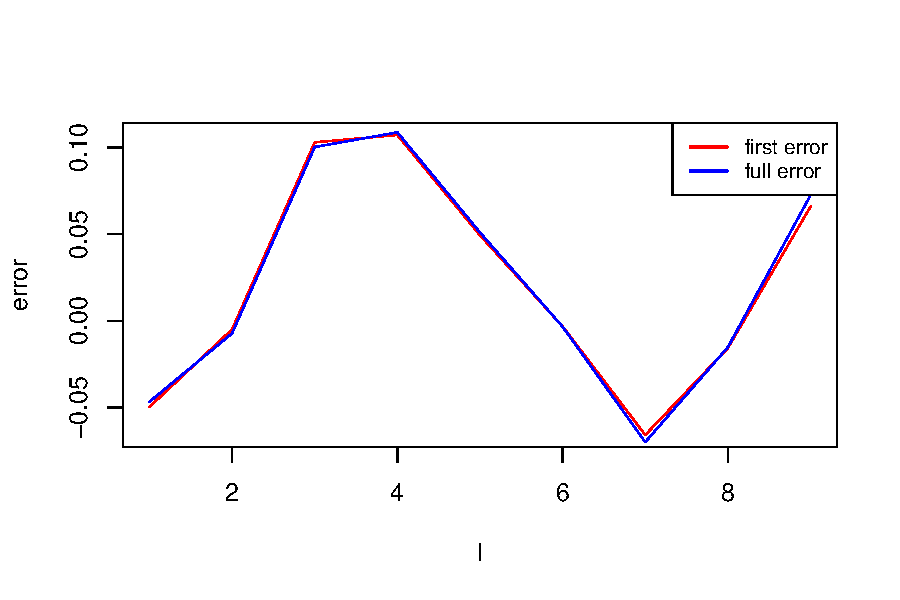
\includegraphics[width=0.6\linewidth]{img/first_vs_full_re.pdf}
		\caption{Вещественные части первого порядка и полной ошибок для $\phi = \pi / 4$.}
		\label{fig:harm_noise_pi_4}
	\end{center}
\end{figure}

\begin{figure}[H]
	\begin{center}
		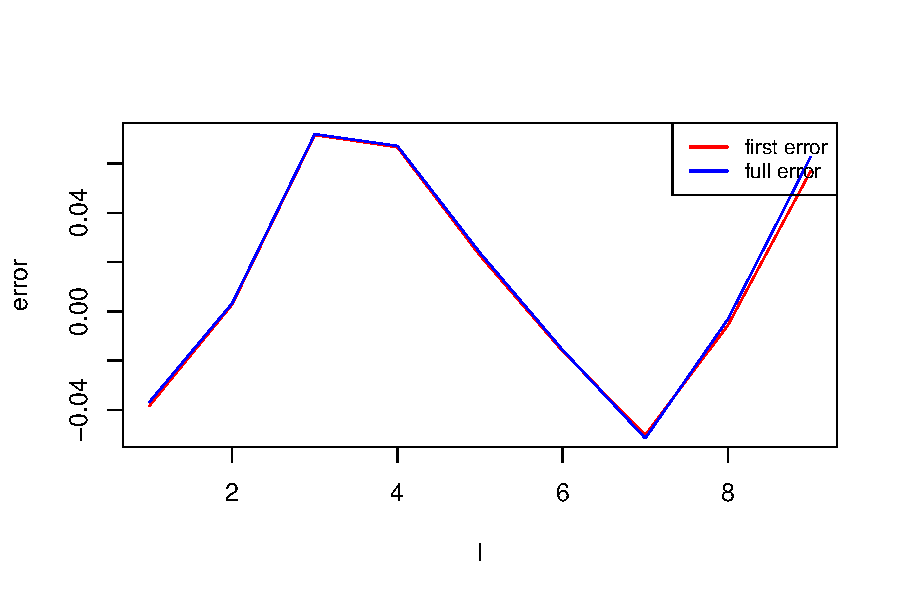
\includegraphics[width=0.6\linewidth]{img/first_vs_full_re_2.pdf}
		\caption{Вещественные части первого порядка и полной ошибок для $\phi = \pi / 2$.}
		\label{fig:harm_noise_pi_2}
	\end{center}
\end{figure}


Из графиков видно, что ошибки практически совпадают даже при маленьких $L$ и $N$, хотя в крайних точках и заметно небольшое расхождение.

Заметим, что в данном случае дисперсии вещественной и мнимой частей возмущения совпадают, а значит и дисперсии вещественной и мнимой частей первого порядка ошибки должны совпадать, ввиду линейности вхождения $\mathbf{E}$ в \eqref{eq:main}.

Показанное совпадение и теорема \ref{th:sum} объясняют, почему в разделе \ref{sec:comp} MSE CSSA было равно сумме MSE SSA для сдвига $\phi = \pi/4$ и равно полусумме MSE SSA для сдвига $\phi = \pi/2$.

\subsection{Случай константных сигналов с выбросом}

Был рассмотрен пример с сигналом $s_l = 1 + \iu 1$ и возмущением в виде выброса $a_1 + \iu a_2 = 10 + \iu 10$ на позиции $k$.

Результаты представлены в таблице~\ref{tab:const_outl_1}, таблице~\ref{tab:const_outl_2}, таблице~\ref{tab:const_outl_ratio}.

\begin{table}[H]
	\begin{center}
		\caption{Максимальное различие первого порядка и полной ошибок при $k = L - 1$.}
		\label{tab:const_outl_1}
		\begin{tabular}{|c|c|c|c|c|}
			\hline
			$N$	& 50 & 100 & 400 & 1600 \\
			\hline
			$L = N / 2$ & 0.1313  & 0.0419  & 0.0033 & 0.0002 \\
			\hline
			$L = 20$ & 0.3074  & 0.1965  & 0.5655 & 0.6720 \\
			\hline
		\end{tabular}
	\end{center}
\end{table}

\begin{table}[H]
	\begin{center}
		\caption{Максимальное различие первого порядка и полной ошибок при $k = N / 2$.}
		\label{tab:const_outl_2}
		\begin{tabular}{|c|c|c|c|c|}
			\hline
			$N$	& 50 & 100 & 400 & 1600 \\
			\hline
			$L = N / 2$ & 7.5e-15  & 5.5e-15  & 3.9e-14 & 4.9e-14 \\
			\hline
			$L = 20$ & 0.5657  & 0.2828  & 0.6364 & 0.6894 \\
			\hline
		\end{tabular}
	\end{center}
\end{table}

\begin{table}[H]
	\begin{center}
		\caption{Отношение ошибок в точке максимального различия, $L = N/2$.}
		\label{tab:const_outl_ratio}
		\begin{tabular}{|c|c|c|c|c|}
			\hline
			$N$	& 50 & 100 & 400 & 1600 \\
			\hline
			$k = 1$ & 0.5  & 0.72  & 0.93 & 0.98 \\
			\hline
			$k = N/4$ & 0.83  & 0.92  & 0.98 & 0.99 \\
			\hline
			$k = N/2 - 1$ & 1.34  & 1.18  & 1.05 & 1.01 \\
			\hline
			$k = N/2$ & 1  & 1  & 1 & 1 \\
			\hline
		\end{tabular}
	\end{center}
\end{table}

Численные результаты показывают, что для случая зашумленных гармоник первый порядок адекватно оценивает полную ошибку восстановления сигнала в каждой точке при любых рассматриваемых параметрах сигналов, хотя на краях заметно небольшое расхождение. 
%(разность ошибок существенно медленнее стремится к нулю).
Однако для случая возмущения в виде выброса это верно, только когда $L$ и $K$ пропорциональны $N$.

%\section{Численное сравнение трудоёмкости}
%
%По теореме \ref{th:sum} нам известно, что для определённого класса рядов, с точки зрения первого порядка ошибки (а из раздела \ref{sec:results} и с точки зрения всей ошибки), SSA эквивалентно CSSA. Поэтому, в данном случае возникает вопрос, какой из методов стоит выбирать? Исходя из этого, в данном разделе мы сравним трудоёмкости методов.
%
%Трудоёмкость методов CSSA и SSA равна трудоёмкости сингулярного разложения (SVD). Мы проведём сравнение трудоёмкостей для пакета \cite{Korobeynikov.etal2014}.
%
%В данном пакете для вещественных рядов SVD вычисляется при помощи метода <<propack>>, для комплексных при помощи пакета <<primme>>. Трудоёмкость метода <<propack>> известна (\cite{Golyandina.etal2018}) и составляет $\mathcal{O}(k N \log(N) + k^2 N)$, где $k$~--- число элементарных компонент, $N$~--- длина ряда. Нас будет интересовать зависимость от $N$ при фикс. $k$, то есть $\mathcal{O}(N \log(N))$.
%
%Отличие метода из <<primme>> заключается в том, что сингулярные числа ищутся для четырёх вещественных матриц, $\Re(\mathbf{X})\Re(\mathbf{X})^\mathrm{T}$, $\Re(\mathbf{X})\Im(\mathbf{X})^\mathrm{T}$, $\Im(\mathbf{X})\Re(\mathbf{X})^\mathrm{T}$, $\Im(\mathbf{X})\Im(\mathbf{X})^\mathrm{T}$, вместо двух $\Re(\mathbf{X})\Re(\mathbf{X})^\mathrm{T}$ и $\Im(\mathbf{X})\Im(\mathbf{X})^\mathrm{T}$ для <<propack>>. Исходя из этого, CSSA в среднем должен работать вдвое медленнее SSA.
%
%Проверим это утверждение на примере. Зашумлённая гармоника
%$$s_l = \cos(2 \pi l / 10) + \iu\cos(2 \pi l / 10 + \phi),$$
%параметры $\sigma^2 = 0.01$, $L = N/2$.
%
%Результаты представлены в таблице \ref{tab:time_comp}
%\begin{table}[H]
%	\begin{center}
%		\caption{Время работы при $k = 2$ и $100$ повторах.}
%		\label{tab:time_comp}
%		\begin{tabular}{|c|c|c|c|}
%			\hline
%			$N$	& 1e3 & 1e4 & 1e5\\
%			\hline
%			CSSA & 2.63 & 6.72 & 71.68\\
%			\hline
%			SSA & 1.10 & 3.98 & 38.92\\
%			\hline
%			CSSA / SSA & 2.39  & 1.69  & 1.84\\
%			\hline
%		\end{tabular}
%	\end{center}
%\end{table}
%
%Из таблицы видно, что время работы отличается приблизительно вдвое. Соответственно, пример подтверждает, что асимптотика по $N$ используемых реализаций CSSA и SSA совпадает, тогда как коэффициенты отличаются вдвое в пользу SSA. Соответственно, с точки зрения времени работы использование SSA предпочтительно, но разница не существенна.

%\chapter{Ошибки восстановления для комплексной экспоненты}
%
%Наиболее распространенным примером сигнала временных рядов для анализа, является сумма комплексных экспонент. Однако, как замечалось ранее, комплексная экспонента, в общем случае, не удовлетворяет условию теоремы $1$, а потому полученные результаты для такого ряда неприменимы.
%
%В связи с этим, в данном разделе рассматриваются примеры комплексной экспоненты и на них проверяется применимость полученных результатов.
%
%%\section{Пример}
%%При построении комплексных робастных методов возникает вопрос: Что считать выбросом? В данной работе выброс считается как элемент с аномально большим модулем. В связи с этим возникает другой вопрос: Не могут ли возникнуть проблемы в случае несимметричности распределения модуля выброса по вещественной и мнимой части? То есть не может ли получиться такой ситуации, что алгоритм посчитает выбросом точку, имеющую очень большое отклонение по вещественной оси, но на мнимой оси эта точка выбросом не является, что приведёт к ухудшению выделения тренда по мнимой оси.
%%
%%Для рассмотрения примера на тему возьмём прошлый ряд, но выбросы сосредоточим только на вещественной оси, их вещественную часть оставив прежней. Так же в данном примере будет осмыслено посчитать помимо совместных ошибок ещё и отдельно ошибки вещественной и мнимой частей.
%%
%%Графики выделения тренда представлены на Рис. \ref{analys_Re_3}, \ref{analys_Im_3}. Результаты RMSE для примера представлены в таблице \ref{tab5}. Так же посчитаем RMSE отдельно для вещественной и мнимой части для прошлого примера, для которого выбросы по модулю сделаем равными текущим, результат в таблице \ref{tab6}.
%%%Значения p-value представлены в таблице \ref{tab: pval5}.
%%
%%\begin{figure}[H]
%%	\begin{center}
%%		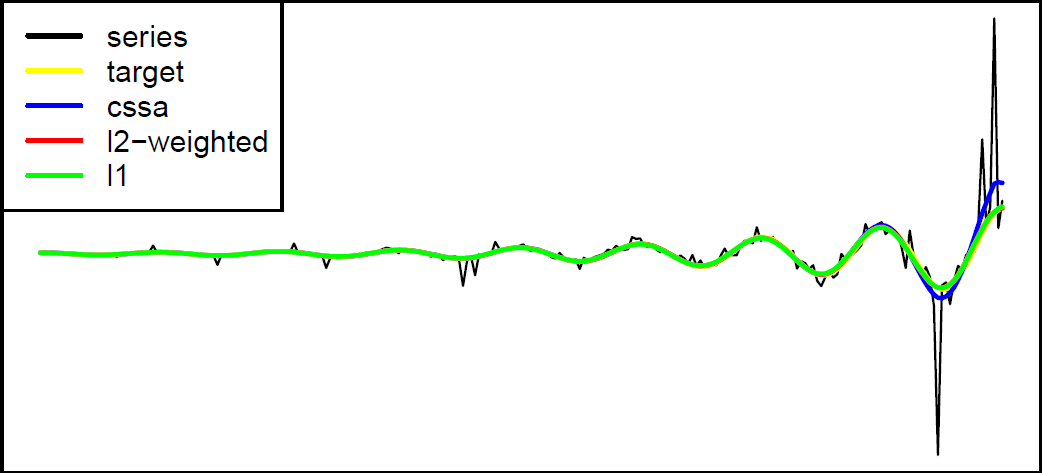
\includegraphics[width=0.67\linewidth]{analys_3_Re.png}
%%		\caption{Вещественная часть выделения тренда несколькими способами.}
%%		\label{analys_Re_3}
%%	\end{center}
%%\end{figure}
%%
%%\begin{figure}[H]
%%	\begin{center}
%%		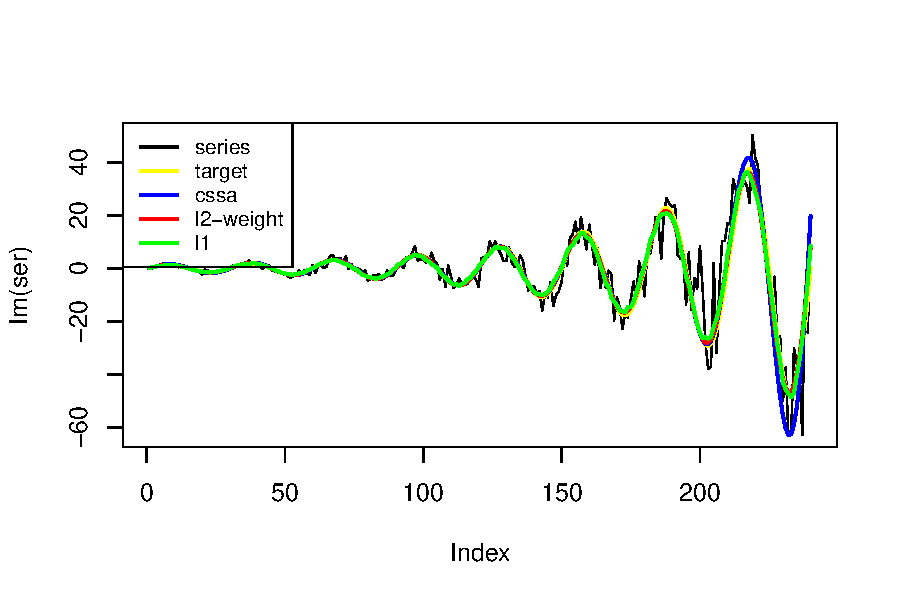
\includegraphics[width=0.67\linewidth]{analys_3_Im.png}
%%		\caption{Мнимая часть выделения тренда несколькими способами.}
%%		\label{analys_Im_3}
%%	\end{center}
%%\end{figure}
%%
%%\begin{table}[H]
%%	\begin{center}
%%		\caption{Оценки RMSE различных методов для $M = 30$ реализаций ряда с вещественными выбросами.}
%%		\label{tab5}
%%		\begin{tabular}{|c|c|c|c|c|c|c|}
%%			\hline
%%			Method 	& CSSA & L1 & weighted L2 & loess L2 & median L2 & lowess L2 \\
%%			\hline
%%			RMSE (совм.) & 3.53  & 1.55  & 1.72 & $\mathbf{1.45}$ & 1.48 & 1.46\\
%%			\hline
%%			RMSE (Re) & 2.63  & 1.06  & 1.23 & $\mathbf{1.05}$ & 1.07 & 1.06\\
%%			\hline
%%			RMSE (Im) & 2.33  & 1.14  & 1.2 & $\mathbf{0.98}$ & 1.02 & 1\\
%%			\hline
%%		\end{tabular}
%%	\end{center}
%%\end{table}
%%
%%\begin{table}[H]
%%	\begin{center}
%%		\caption{Оценки RMSE различных методов для $M = 30$ реализаций прошлого примера.}
%%		\label{tab6}
%%		\begin{tabular}{|c|c|c|c|c|c|c|}
%%			\hline
%%			Method 	& CSSA & L1 & weighted L2 & loess L2 & median L2 & lowess L2 \\
%%			\hline
%%			RMSE (совм.) & 3.53  & 1.29  & 1.34 & $\mathbf{0.97}$ & 1 & 0.98\\
%%			\hline
%%			RMSE (Re) & 2.5  & 0.85  & 0.95 & $\mathbf{0.7}$ & 0.71 & $\mathbf{0.7}$\\
%%			\hline
%%			RMSE (Im) & 2.5  & 0.97  & 0.95 & $\mathbf{0.69}$ & 0.71 & $\mathbf{0.7}$\\
%%			\hline
%%		\end{tabular}
%%	\end{center}
%%\end{table}
%%
%%%\begin{table}[H]
%%%	\caption{p-value для сравнения различных методов с наилучшим с выбросами.}
%%%	\label{tab: pval5}
%%%	\begin{center}
%%%		\begin{tabular}{|c|c|c|c|c|c|}
%%%			\hline
%%%			Method & CSSA	& L1 & weighted L2 & median L2 & lowess L2  \\
%%%			\hline
%%%			loess L2 (совм.) & 1.1e-08  & \textbf{0.166} &  0.028  & \textbf{0.46} & \textbf{0.756}  \\
%%%			\hline
%%%			loess L2 (Re) & 1.4e-08  & \textbf{0.69} &  \textbf{0.073}  & \textbf{0.54} & \textbf{0.8}  \\
%%%			\hline
%%%			loess L2 (Im) & 3e-08  & 0.0014 &  0.001  & \textbf{0.19} & \textbf{0.26}  \\
%%%			\hline
%%%		\end{tabular} \\
%%%	\end{center}
%%%\end{table}
%%
%%Получаем, что общая ошибка в случае, когда выбросы равномерно распределены по вещественной и по мнимой оси ниже, но распределение ошибок по вещественной и мнимой осям сохраняется. Что свидетельствует в пользу нашего предположения и кажется разумным для данных методов, как для методов, приближающих весь комплексный ряд, а не вещественную и мнимую части по отдельности.
%
%
%\section{Вещественные выбросы}
%
%Рассмотрим случай вещественных выбросов для комплексной экспоненты. Попробуем проверить результат теоремы \ref{th:sum} для этого случая на примере.
%
%Будем рассматривать экспоненту без шума, длины $N = 240$
%$$x_n = e^{4n/N} e^{2n\pi/30i}.$$
%с $5\%$ выбросов вида $5 \Re(x_i)$.
%
%Графики ряда представлены на Рис. \ref{ser_Re_5}, \ref{ser_Im_5}.
%
%\begin{figure}[H]
%	\begin{center}
%		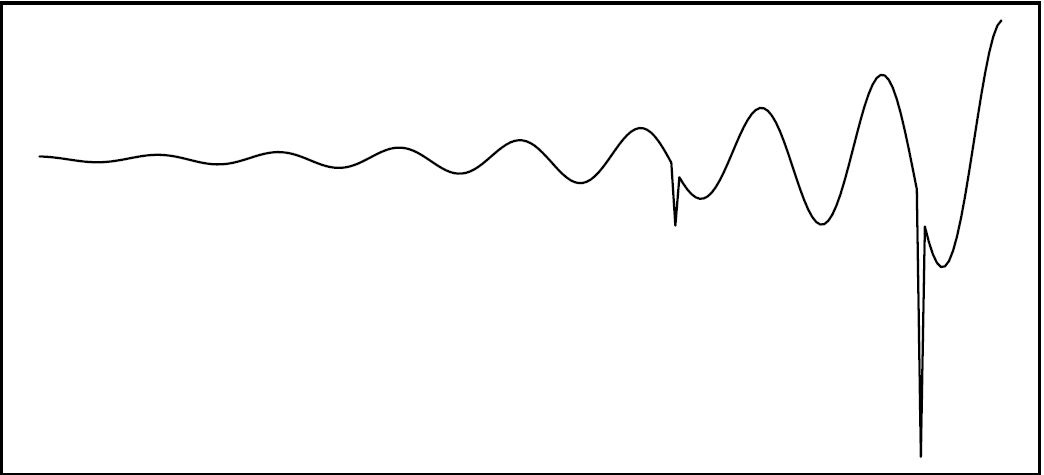
\includegraphics[width=0.67\linewidth]{Re_outl_Re.png}
%		\caption{График вещественной части ряда.}
%		\label{ser_Re_5}
%	\end{center}
%\end{figure}
%
%\begin{figure}[H]
%	\begin{center}
%		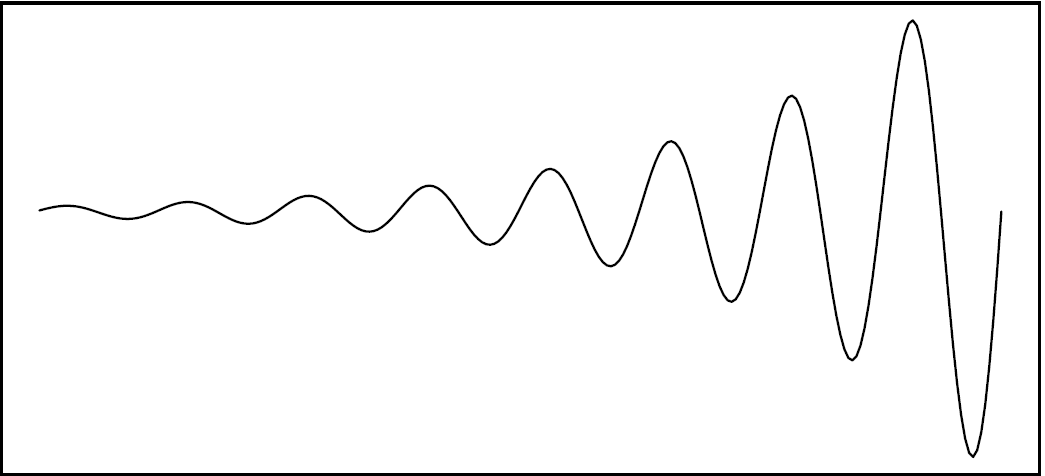
\includegraphics[width=0.67\linewidth]{Re_outl_Im.png}
%		\caption{График мнимой части ряда.}
%		\label{ser_Im_5}
%	\end{center}
%\end{figure}
%
%
%%\subsection{Модификация функции весов}
%%
%%У этого ряда все выбросы находятся в вещественной части. Разумно воспользоваться этой информацией и при идентификации выбросов смотреть лишь на вещественную часть, чтобы уменьшить ошибку.
%%
%%В выбранной нами в данной работе функции весов выброс идентифицируется по модулю числа. Первое, что приходит на ум~--- модифицировать функцию весов, чтобы она реагировала исключительно на вещественную часть. Тогда получаем
%%$$w(x) =
%%\begin{cases}
%%	(1 - (\frac{|\Re(x)|}{\alpha})^2)^2 &|\Re(x)| \leq \alpha\\
%%	0 &|\Re(x)| > \alpha\\
%%\end{cases}.$$
%%
%%Проведём сравнение ошибок двух алгоритмов, с $|x|$ и $|\Re(x)|$ для предложенного примера. Результаты в таблице \ref{tab7}, ошибки приведены отдельно для всего ряда, вещественной и мнимой частей.
%%
%%\begin{table}[H]
%%	\begin{center}
%%		\caption{сравнения RMSE}
%%		\label{tab7}
%%		\begin{tabular}{|c|c|c|c|}
%%			\hline
%%			Ряд & w-L2 abs & w-L2 Re & p-value \\
%%			\hline
%%			complex & 0.053  & 0.053 & 0.62 \\
%%			\hline
%%			Re & 0.037  & 0.037 & 0.56 \\
%%			\hline
%%			Im & 0.38  & 0.038 & 0.69 \\
%%			\hline
%%		\end{tabular}
%%	\end{center}
%%\end{table}
%%
%%Получили, что модификация не дала прироста в ошибке даже по вещественной оси.
%
%Для данного ряда рассмотрим $\Re(f^{(1)})$ и $\Im(f^{(1)})$, проверим, ведут ли они себя так же, как $f^{(1)*}_{\Re}$ и $f^{(1)*}_{\Im}$.
%
%Графики $\Re(f^{(1)})$ и $\Im(f^{(1)})$ приведены на Рис. \ref{f1}.
%
%\begin{figure}[H]
%	\begin{center}
%		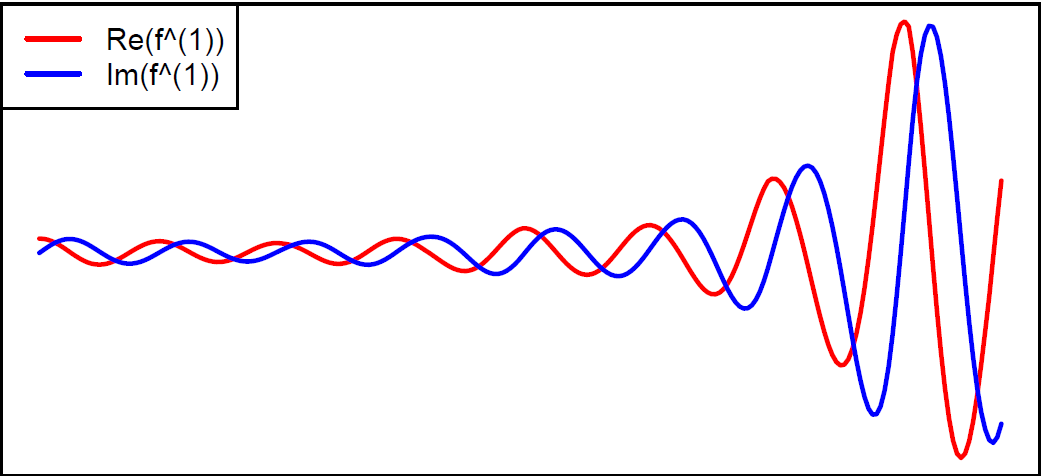
\includegraphics[width=0.67\linewidth]{f1.png}
%		\caption{Графики $\Re(f^{(1)})$ и $\Im(f^{(1)})$.}
%		\label{f1}
%	\end{center}
%\end{figure}
%
%По представленным графикам видно, что вещественная и мнимая части ошибки восстановления ведут себя одинаково, тогда как $f^{(1)*}_{\Im} = 0$, а $f^{(1)*}_{\Re} \neq 0$ из-за того, что все выбросы в вещественной части. Получаем, что результат теоремы \ref{th:sum} не выполняется для общего случая комплексной экспоненты.
%
%
%%\section{Инвариантное по RMSE преобразование}
%%
%%В разделе \ref{ss:RMSEinv} был найден инвариант по RMSE для рядов, удовлетворяющих теореме \ref{th:sum}.
%%
%%Проверим, является ли преобразование, сохраняющее модули, инвариантом по RMSE для случая комплексной экспоненты
%%
%%Рассмотрим ряд с растущей амплитудой и шумом непостоянной дисперсии.
%%Длину ряда возьмем $N = 240$
%%$$x_n = e^{4n/N} e^{2n\pi/30i} + \frac{1}{2}e^{4n/N} \varepsilon_n, ~ \varepsilon_n \sim CN(0,1).$$
%%и $5\%$ выбросов с величиной выброса $4x_i$.
%%
%%Графики ряда представлены на Рис. \ref{ser_Re_3}, \ref{ser_Im_3}.
%%
%%\begin{figure}[H]
%%	\begin{center}
%%		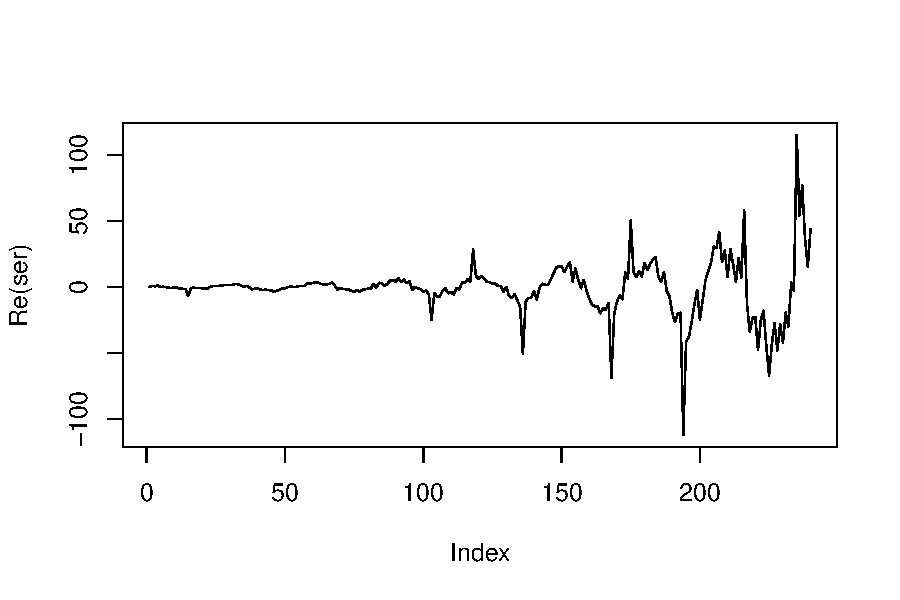
\includegraphics[width=0.67\linewidth]{ser_3_Re.png}
%%		\caption{График вещественной части ряда.}
%%		\label{ser_Re_3}
%%	\end{center}
%%\end{figure}
%%
%%\begin{figure}[H]
%%	\begin{center}
%%		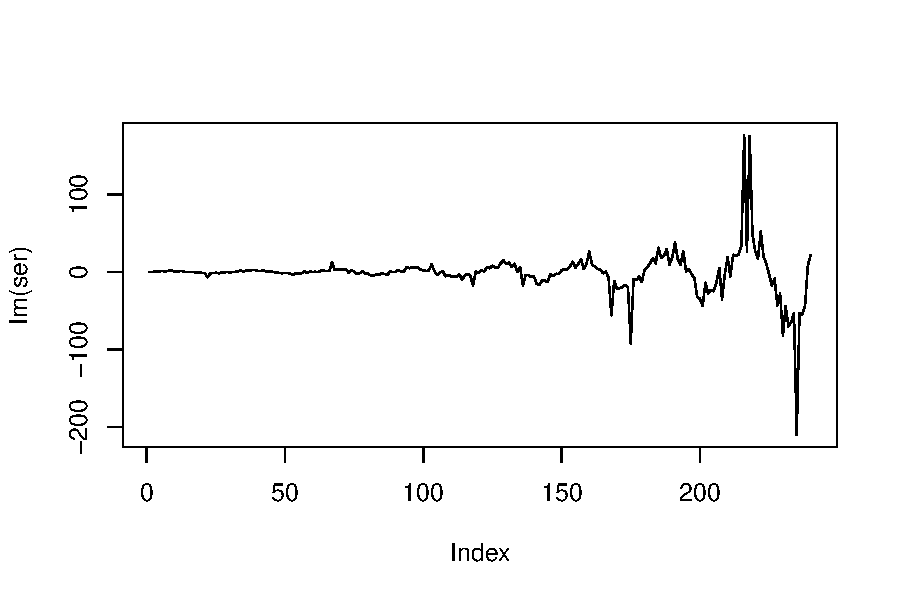
\includegraphics[width=0.67\linewidth]{ser_3_Im.png}
%%		\caption{График мнимой части ряда.}
%%		\label{ser_Im_3}
%%	\end{center}
%%\end{figure}
%%
%%Теперь поймем, какое преобразование сохраняет модуль, найдем вещественное $c_i$ такое, что\\
%%$|x_i + c_i| = |x_i + 4 x_i|$.
%%
%%Пусть $\Re(x_i) = a_i$, $\Im(x_i) = b_i$, тогда
%%$$\sqrt{(c_i + a_i)^2 + b_i^2} = \sqrt{25 a_i^2 + 25 b_i^2}$$
%%$$(c_i + a_i)^2 = 25 a_i^2 + 24 b_i^2$$
%%$$|c_i| = \sqrt{25 a_i^2 + 24 b_i^2} - a_i$$
%%
%%Не умаляя общности, можно рассмотреть знак $c_i$, совпадающим с $x_i$.
%%Тогда рассмотрим тот же ряд с $5\%$ выбросов, но с величиной выброса $\sign(x_i)(\sqrt{25 \Re(x_i)^2 + 24 \Im(x_i)^2} - \Re(x_i))$.
%%
%%Графики ряда представлены на Рис. \ref{ser_Re_4}, \ref{ser_Im_4}.
%%
%%\begin{figure}[H]
%%	\begin{center}
%%		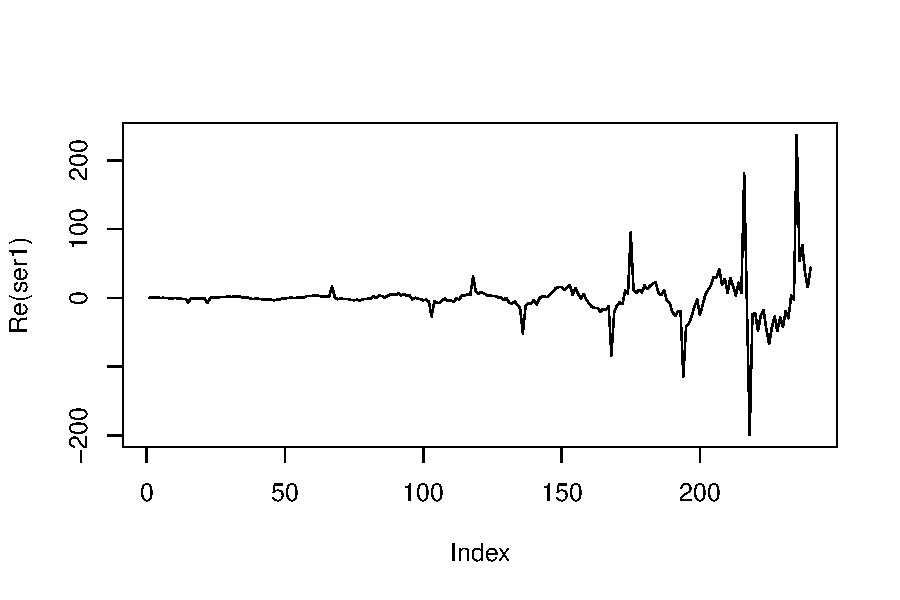
\includegraphics[width=0.67\linewidth]{ser_4_Re.png}
%%		\caption{График вещественной части ряда.}
%%		\label{ser_Re_4}
%%	\end{center}
%%\end{figure}
%%
%%\begin{figure}[H]
%%	\begin{center}
%%		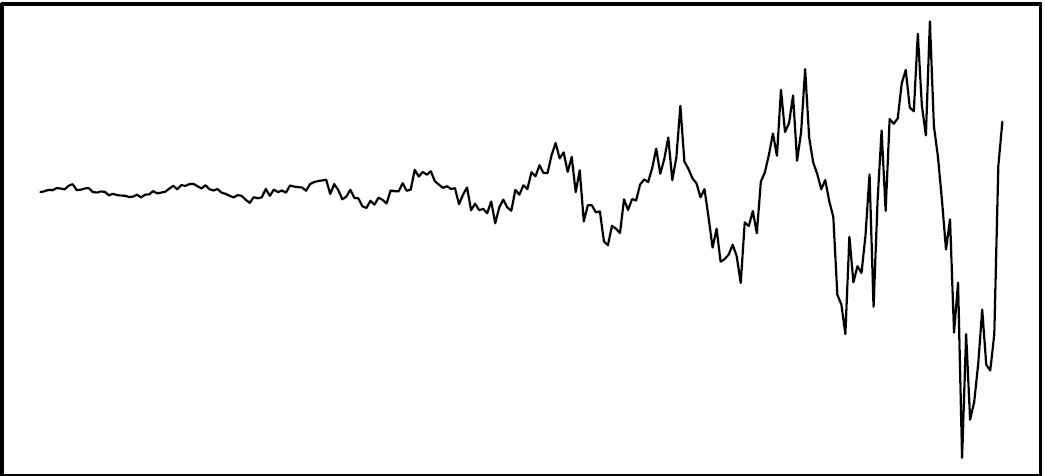
\includegraphics[width=0.67\linewidth]{ser_4_Im.png}
%%		\caption{График мнимой части ряда.}
%%		\label{ser_Im_4}
%%	\end{center}
%%\end{figure}
%%
%%
%%Результаты сравнений RMSE на двух рядах приведены в таблице \ref{pvaltab}.
%%
%%\begin{table}[H]
%%	\begin{center}
%%		\caption{p-value сравнения RMSE}
%%		\label{pvaltab}
%%		\begin{tabular}{|c|c|c|c|c|}
%%			\hline
%%			Ряд  & CSSA & L1 & w-L2 & mod. w-L2 \\
%%			\hline
%%			complex & 0.0045 & 0.51  & 0.65 & 0.56 \\
%%			\hline
%%			Re & 0.06 & 0.43 & 0.64 & 0.46 \\
%%			\hline
%%			Im & 0.0002 &0.57  & 0.66 & 0.72 \\
%%			\hline
%%		\end{tabular}
%%	\end{center}
%%\end{table}
%%
%%Как мы видим, гипотеза о различии RMSE на двух рядах значима для CSSA, особенно для мнимой части, то есть данное преобразование не является инвариантом для CSSA в случае комплексной экспоненты.
%%
%%Для остальных методов гипотеза незначима. То есть преобразование, сохраняющее модули, является инвариантом. Можно предположить, что это связано с тем, что в каждом из них выброс идентифицируется по своему модулю.


\conclusion
%\section{Заключение}
В работе были рассмотрены обобщения двух робастных вариантов метода SSA на комплексно-значный случай.
Был проведён обзор двух известных подходов к построению робастных версий SSA для вещественных рядов: замена проекции по норме в $\mathbb{L}_2$ на проекцию по норме в $\mathbb{L}_1$ и на взвешенную проекцию по норме в $\mathbb{L}_2$ и их имплементация для комплексного случая.
%В предположении, что число итераций не зависит от длины ряда, было произведено сравнение трудоёмкостей методов. Метод %проекции на $\mathbb{L}_1$ оказался наименее трудоёмким.
Работа методов была показана на нескольких примерах, подтверждающих эффективность робастных модификаций, в сравнении с базовым вариантом метода CSSA для рядов с выбросами. Все рассматриваемые модификации были реализованы на R.

В работе удалось получить теоретические результаты о сравнении первого порядка ошибки CSSA и SSA, применимые, в основном, к рядам с совпадающими траекторным пространствами. Основной из полученных результатов, сформулированный в виде теоремы, гласит, что для таких рядов первый порядок ошибки восстановления для CSSA выражается как сумма первых порядков для SSA, применённого отдельно к вещественной и мнимой частям ряда.

Удалось подвести теоретическую базу под имеющиеся ранее численные результаты (\cite{Golyandina.etal2013}) по сравнению CSSA и SSA для двух зашумленных гармоник с одинаковой частотой и сдвигом, не кратным $\pi/2$. Для зашумленной комплексной экспоненты был численно получен более общий, нежели имеющиеся ранее, численный результат.
Результаты показывают, что только в случае сигнала в виде комплексной экспоненты применение CSSA имеет смысл с точки зрения уменьшения ошибки восстановления сигнала.

Для константного ряда с выбросами был получен явный вид первого порядка ошибок оценки сигнала в каждой точке.

Для обоих случаев было численно исследовано соотношение между первым порядком ошибки и полной ошибкой.
В случае случайного возмущения оказалось, что первый порядок ошибки практически совпадает с полной ошибкой. Однако в случае неслучайного возмущения выбросом это не так и требуются дополнительные условия на пропорциональность длины окна $L$ длине ряда $N$.


%\nocite{*}
\bibliographystyle{ugost2008}
\bibliography{literature}

\end{document}
